\documentclass[a4paper, 12pt]{scrartcl}

\usepackage{scrpage2}
\usepackage[left=2.5cm,right=2.5cm, top=3cm, bottom=4cm]{geometry}
\usepackage[utf8]{inputenc}
\usepackage[ngerman]{babel}
\usepackage[T1]{fontenc}
\usepackage{amsmath}
\usepackage{amssymb}
\usepackage{amsfonts}

\usepackage{graphicx}

\usepackage{float}
\usepackage{adjustbox}
\usepackage{hyperref}
\usepackage{textcomp}
\usepackage{multirow}
\usepackage{array}

%\usepackage{enumerate}
\usepackage[shortlabels]{enumitem}

% Einrücken verhindern
\setlength{\parindent}{0em} 


\begin{document}


\begin{titlepage}
	\centering
	{\Huge\bfseries Versuchsprotokoll\par}
	\vspace{2cm}
	{\scshape\LARGE Akustik \par}
	\vspace{1cm}
	{\Large Schallgeschwindigkeit in Festkörpern \\ und die Physik der Gitarre\par}
	\vfill
	{\large\itshape Simon Schwarz und Marius Ising\par}

	\vfill
\end{titlepage}

\tableofcontents
\newpage

\section{Schallgeschwindigkeit in Festkörpern}


\subsection{Versuchsbeschreibung}

Das Ziel des folgenden Versuchs ist die Bestimmung der Schallgeschwindigkeit und des Elastizitätsmoduls von vier verschiedenen Metallen. Das Elastizitätsmodul 
$$E = \frac{F/A}{\Delta L/L}$$
ist eine Materialkonstante und gibt die relative Längenausdehnung in Abhängigkeit von der angreifenden Zugspannung an. Eine Messung ist über die Ausbreitungsgeschwindigkeit 
$$v_l = \sqrt{\frac{E}{\rho}}$$
möglich, wobei $\rho$ die Dichte des Materials bezeichnet. Die dynamische Bestimmung von $E$ durch das direkte Messen der Längenausdehnung ist bei Metallstäben nicht praktikabel, da für Metalle $E$ in der Größenordnung $10^{11} N/m^2$ liegt. Der Metallstab hat als Zylinder mit Länge $L$, Durchmesser $D$ und Masse $M$ die Dichte
\begin{equation}\label{eq:rho}
\rho = \frac{4M}{\pi LD^2}\text{,}
\end{equation}
so dass sich mit
\begin{equation}\label{eq:ges}
v_l = 2L f_0
\end{equation}
das Elastizitätsmodul
\begin{equation}\label{eq:ela}
E = 16 f_0^2 LM \frac{1}{\pi D^2}
\end{equation}
ergibt. Dabei ist $f_0$ die Grundfrequenz der longitudinalen Schallwelle, die neben den Größen $L$, $D$ und $M$ experimentell bestimmt werden soll.

\subsection{Versuchsaufbau}

Folgende Geräte werden für den Versuch benötigt: Zwei Tischklemmen, eine Kreuzmuffe, eine Metallstange $\sim 20$ cm, ein Metallstift, ein Metallstift, ein Sensor-Cassy mit Laptop, ein Mikrofon, ein Gummihammer, eine Waage, ein Bandmaß, eine Mikrometerschraube und vier Metallstangen $\sim 130$cm (Kupfer, Stahl, Aluminium und Messing).

\begin{figure}[h]
	\centering
	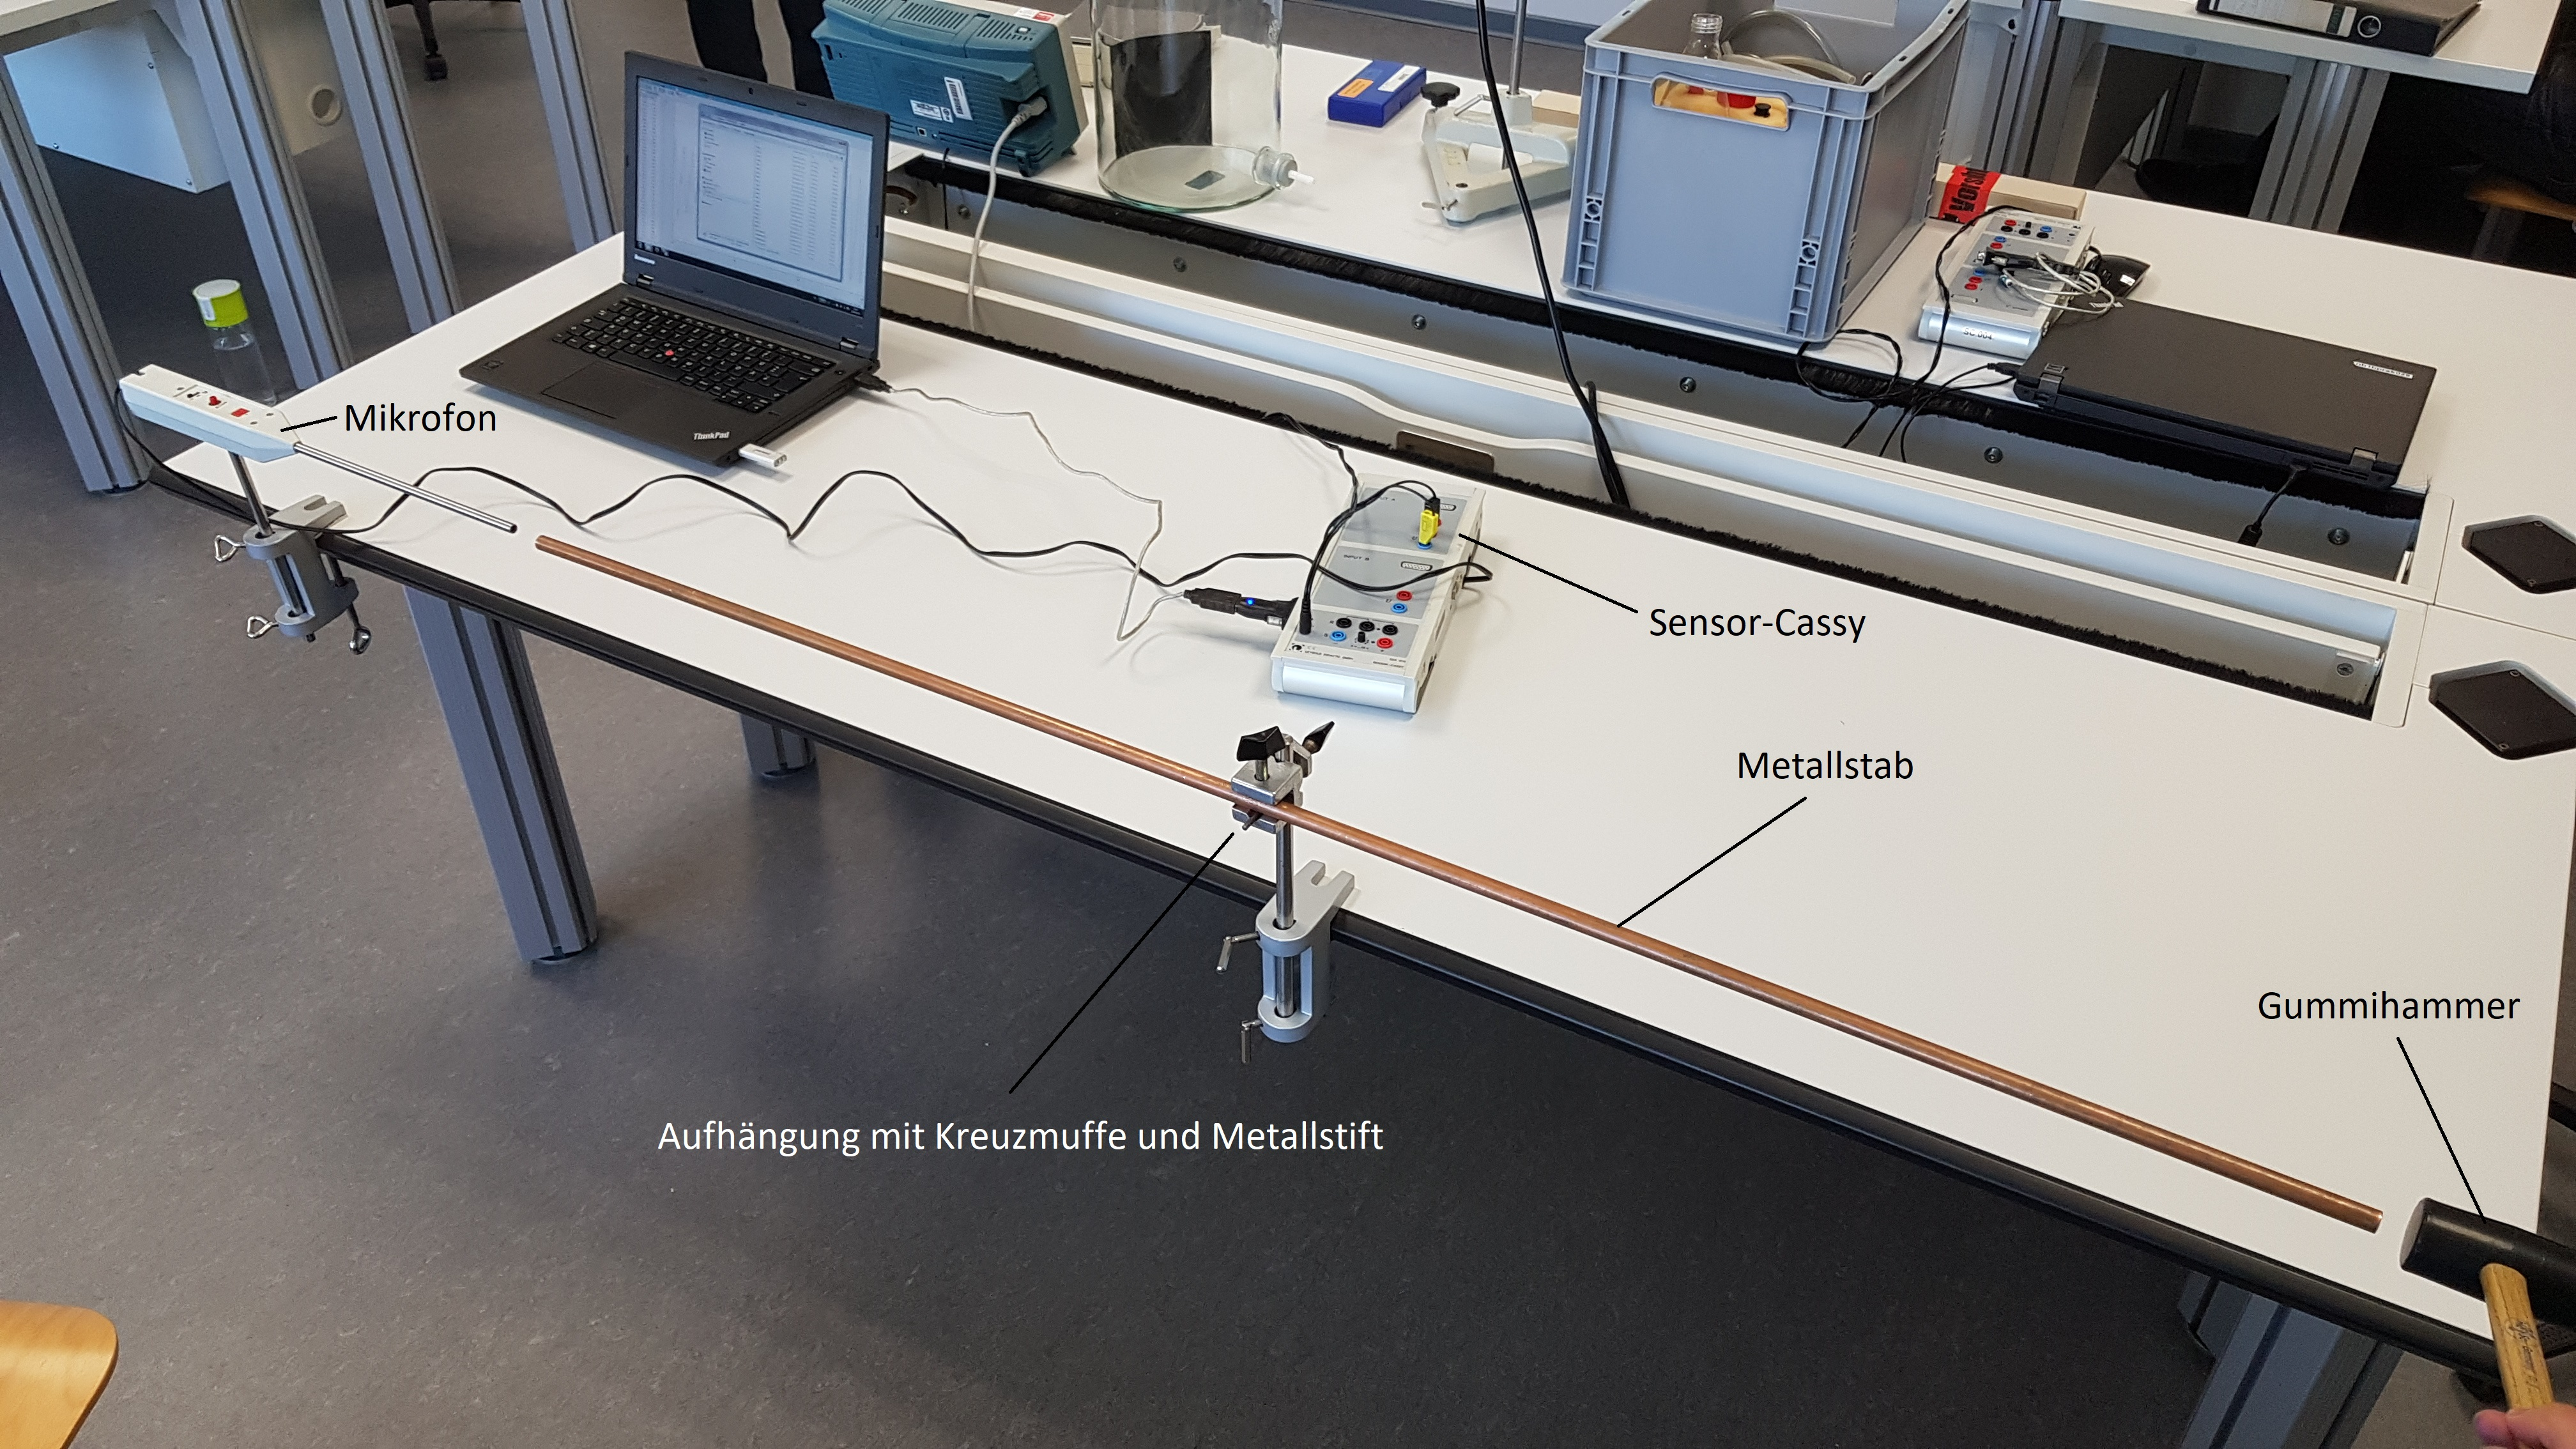
\includegraphics[width=\linewidth]{bilder/aufbau_festkoerper.jpg}
	\caption{Versuchsaufbau}
\end{figure}

Eine große, zu untersuchende Metallstange wird mit Hilfe einer Tischklemme, der kleinen Metallstange und der Kreuzmuffe horizontal am Tisch befestigt. Dabei muss die Stange mittig an zwei Punkten eingespannt werden, damit die Schwingung nicht beinträchtigt wird. Dies ist in Abbildung \ref{pic:aufhaengung} dargestellt. In kleinem Abstand zu einem Ende der großen Metallstange wird das Mikrofon platziert, das den Schalldruck und somit die Schallwellen misst. Das Mikrofon ist am Sensor-Cassy angeschlossen. Am anderen Ende kann die Stange durch einen Schlag mit dem Gummihammer in Schwingung versetzt werden.

\begin{figure}[H]
	\centering
	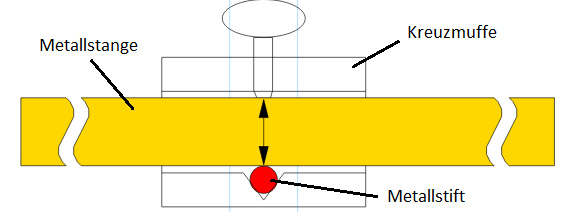
\includegraphics[width=\linewidth]{bilder/aufhaengung_beschriftet.png}
	\caption{Aufhängung der Metallstange an zwei Punkten mit der Kreuzmuffe und einem Metallstift}
	\label{pic:aufhaengung}
\end{figure}



\subsection{Versuchsdurchführung}

Die Stäbe werden nacheinander ausgemessen und in die Versuchsvorrichtung eingespannt. Für die Länge wird das Maßband verwendet und für die Masse die Waage. Um den Durchmesser zu bestimmen, wird mit einer Mikrometerschraube an verschiedenen Stellen mit verschiedenen Orientierungen gemessen, da der Durchmesser variieren und eine Elliptizität nicht ausgeschlossen werden kann. Ist der Stab eingespannt und das Mikrofon eigeschaltet und ausgerichtet, kann der Stab durch einen Schlag mit dem Gummihammer in Schwingung versetzt werden. Der Schlag sollte möglichst gerade auf das Ende der Stange erfolgen, um transversale Schwingungen des Stabes zu vermeiden. Für jeden Stab wird die Messung fünfach durchgeführt. Bei den vorliegenden Messungen für die Stäbe 5 (Kupfer), 6 (Messing) und 9 (Aluminium) hatte das Seonsor-Cassy die Messparameter:
\begin{enumerate}[-]
\item Messbereich: $-3$ bis $3\,$V
\item Intervall: $100\,\mu$s
\item Messungen: $16000$
\item Messzeit: $1.6\,$s
\end{enumerate}
Da die gemessene Schwingung des Stahlstabes deutlich schneller abgeklungen ist als die der anderen Stäbe, wurden für die Messungen bei Stab 11 (Stahl) die Messparameter
\begin{enumerate}[-]
\item Messbereich: $-3$ bis $3\,$V
\item Intervall: $50\,\mu$s
\item Messungen: $16000$
\item Messzeit: $0.8\,$s
\end{enumerate}
verwendet.

\subsection{Versuchsauswertung}

Für die Messungen der Längen und Massen ergaben sich folgende Werte:

\begin{table}[H]
\centering
\begin{tabular}{cc|c|c|c}
Stabnummer & Material & $L$ [cm] & $M$ [g] & $\overline{D}$ [mm] \\
\hline
$5$ & Kupfer & $129.90\pm 0.07$ & $1295.00\pm 0.03$ & $11.991 \pm 0.081$ \\
$6$ & Messing & $130.00 \pm 0.07$ & $1237.20 \pm 0.03$ & $11.978 \pm 0.005$ \\
$9$ & Aluminium & $129.90 \pm 0.07$ & $407.30 \pm 0.03$ & $11.944 \pm 0.031$ \\
$11$ & Stahl & $130.10 \pm 0.07$ & $1157.60 \pm 0.03$ & $11.989 \pm 0.045$
\end{tabular}
\end{table}
Als Fehler in $\overline{D}$ wurde die Wurzel der empirischen Varianz und nicht die Standardabweichung des arithmetischen Mittels genommen, weil diese den Unebenheiten des Stabes nicht gerecht wird. In Abbildung \ref{pic:rohdaten} ist eine Messung des für den Kupferstab abgebildet.

\begin{figure}[h]
	\centering
	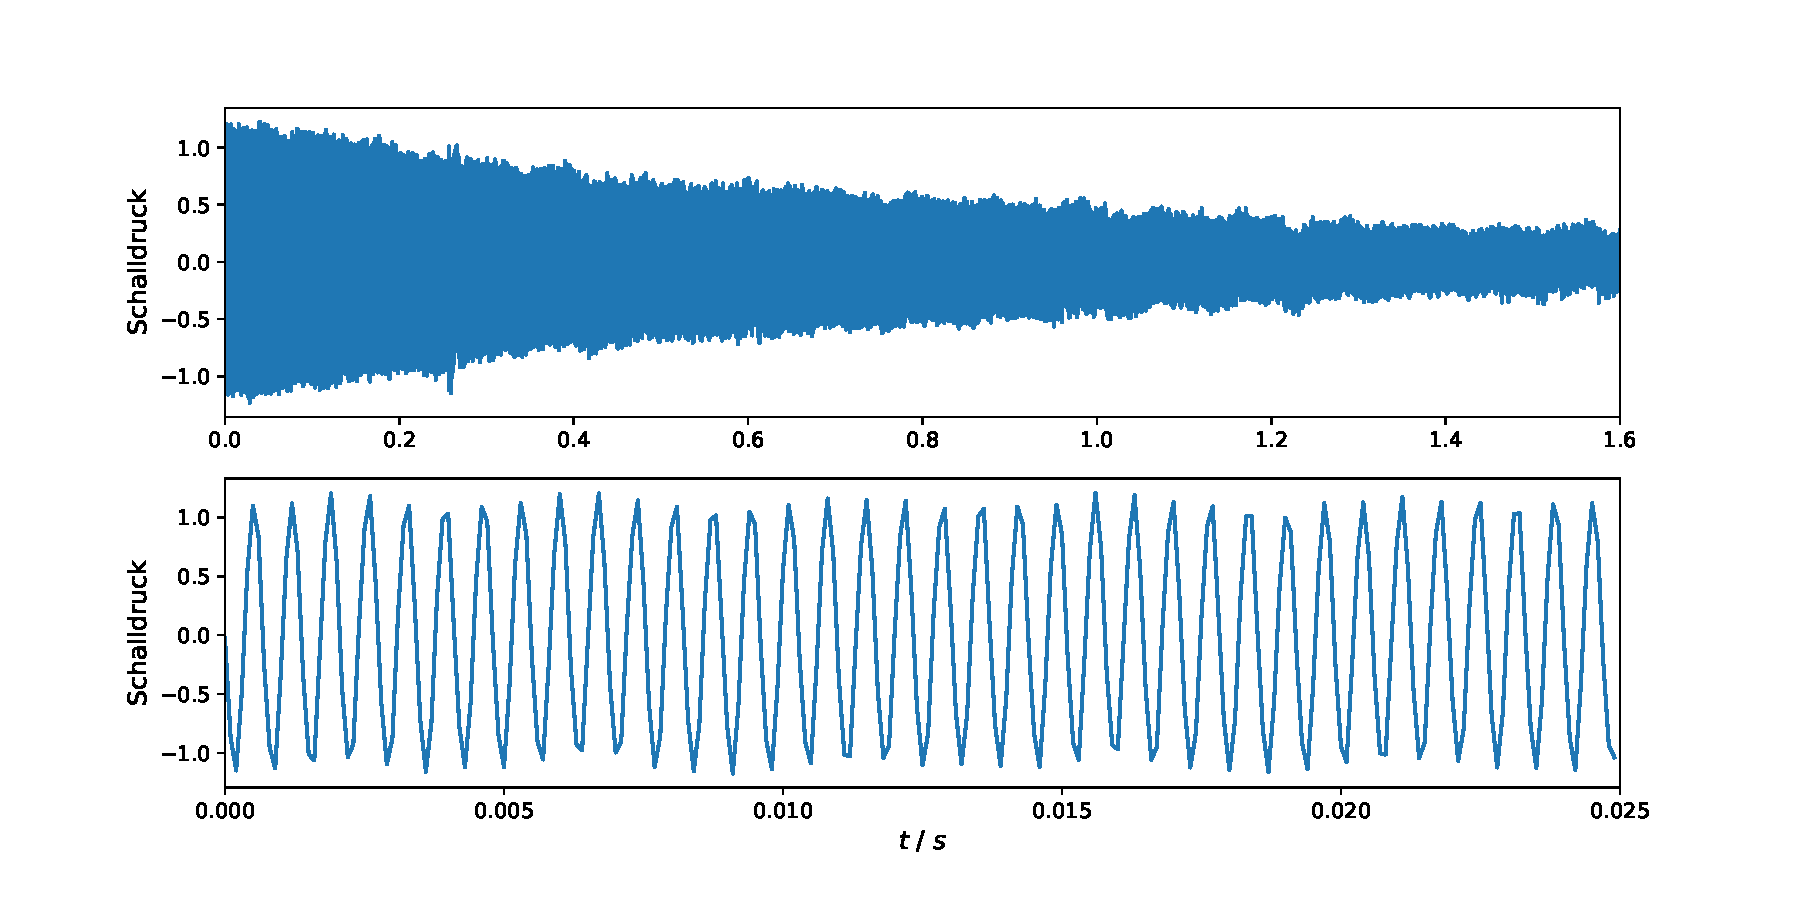
\includegraphics[width=\linewidth]{plots/rohdaten.pdf}
	\caption{Visualisierung der Rohdaten aus der ersten Messung für Stab 5 (\mbox{``Nr5\_1.lab''}) mit zwei verschiedenen Zeitskalen.}
	\label{pic:rohdaten}
\end{figure}

Die Bestimmung von $f_0$ erfolgt mit Hilfe der Frequenzspektren, die durch eine FFT aus den Rohdaten berechnet wird. Das Spektrum für die Schwingung aus Abbildung \ref{pic:rohdaten} ist beispielhaft in Abbildung \ref{pic:spektrum1} dargestellt. Man sieht deutlich die Grundschwingung bei circa $1500$Hz.

\begin{figure}[H]
	\centering
	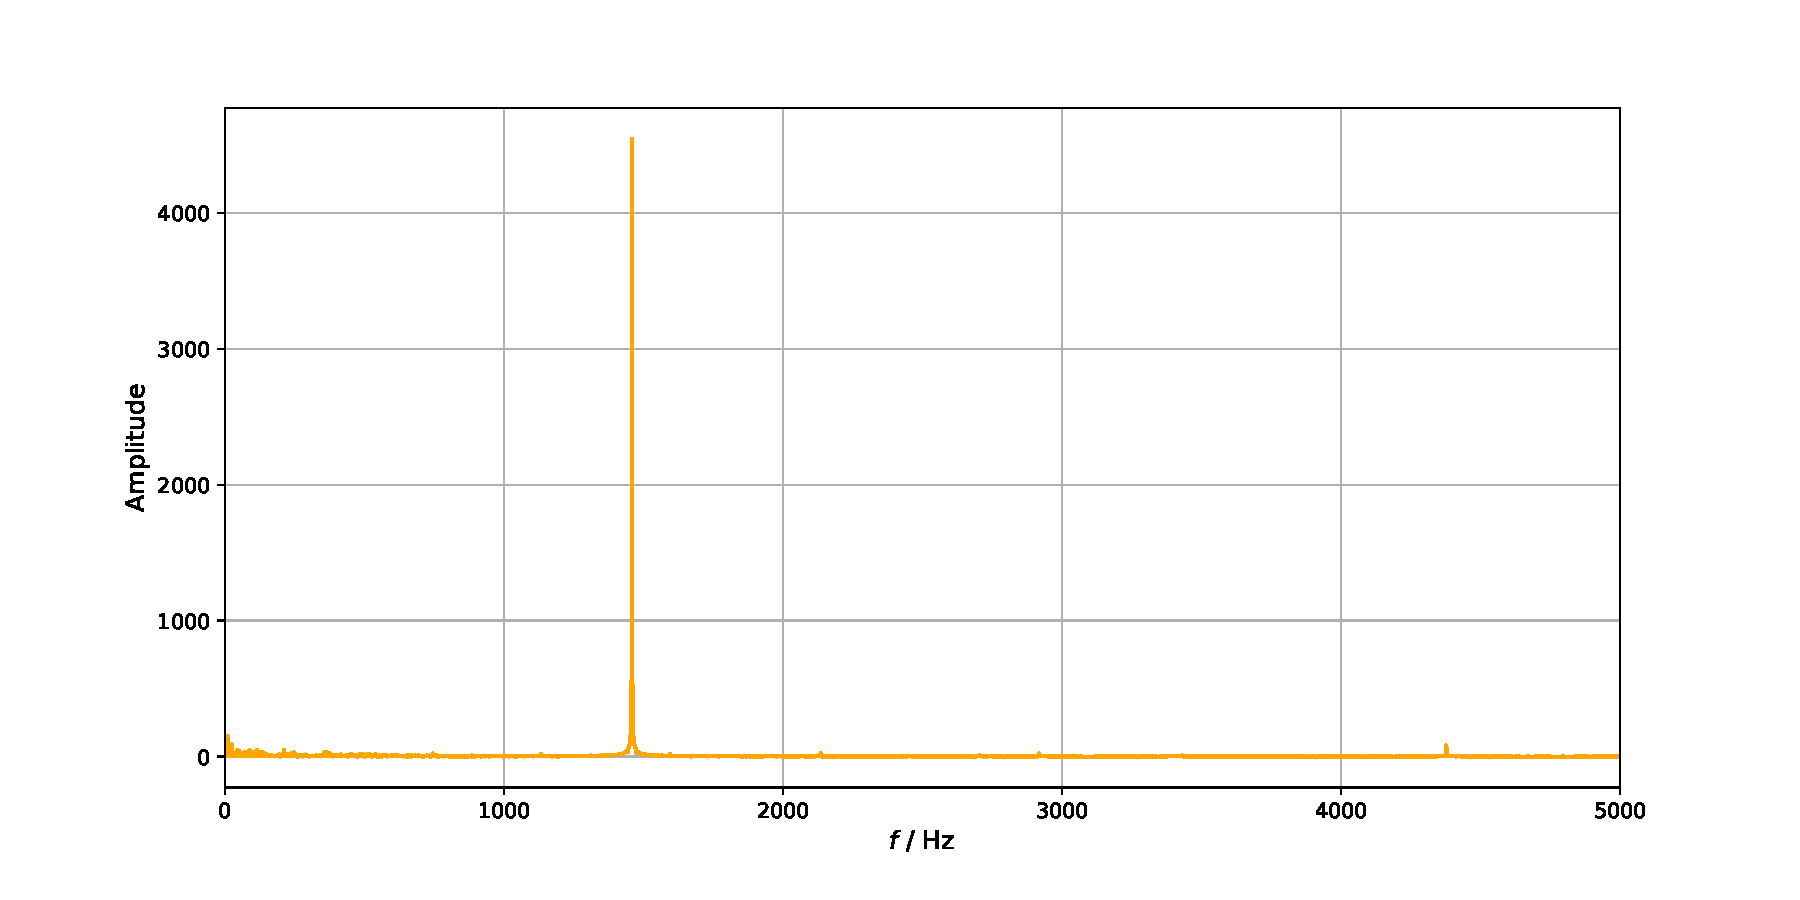
\includegraphics[width=\linewidth]{plots/spektrum1.pdf}
	\caption{Visualisierung des Spektrums der ersten Messung für Stab 5 (\mbox{``Nr5\_1.lab''}) berechnet mittels FFT.}
	\label{pic:spektrum1}
\end{figure}

Um $f_0$ möglichst exakt aus diesem Spektrum ablesen zu können, wird die Peakfinder-Methode aus dem Praktikumspaket verwendet. Für das Spektrum in Abbildung \ref{pic:spektrum1} ist dies in Abbildung \ref{pic:spektrum2} visualisiert. Im Anhang \ref{anhang:plot} finden sich für alle Messungen entsprechende Plots. Als Fehler, der durch das Ablesen, durch die FFT und durch Messunsicherheiten verursacht wird, wird $\sigma_{f} = 0.5\,$Hz verwendet. Als Fehler der Mittelwerte wird der innere Fehler 
$$\sigma_{f_0} = \frac{\sigma_{f}}{\sqrt{5}} = 0.224\,\text{Hz}$$
gewählt, da dieser größer ist als der äußere.

\begin{figure}[H]
	\centering
	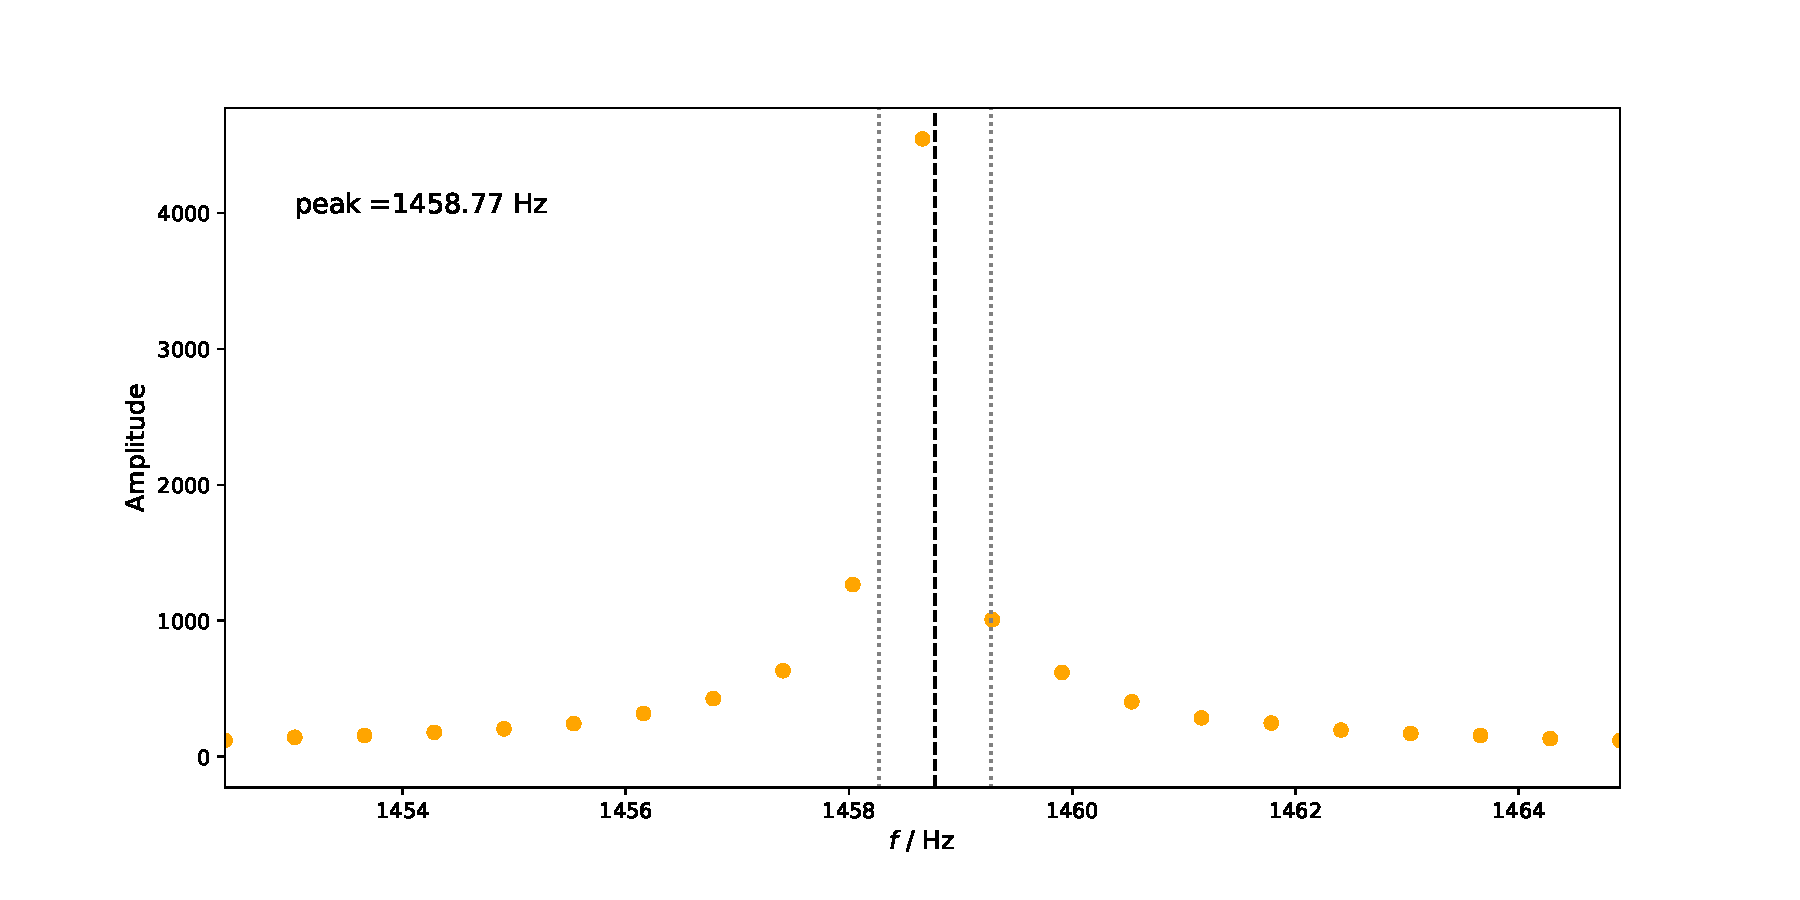
\includegraphics[width=\linewidth]{plots/spektrum2.pdf}
	\caption{Eingezeichnetes Ergebnis der Peakfinder-Methode (in schwarz) mit $\pm0.5\,$Hz (in grau) für das Spektrum der ersten Messung, Stab 5 (\mbox{``Nr5\_1.lab''}).}
	\label{pic:spektrum2}
\end{figure}

Daraus ergeben sich die folgenden Grundfrequenzen:

\begin{table}[H]
\centering
\begin{tabular}{cc|c}
Stabnummer & Material & $\overline{f}_0$ [Hz]\\
\hline
$5$ & Kupfer & $1458.810\pm 0.224$ \\
$6$ & Messing & $1348.122\pm 0.224$\\
$9$ & Aluminium & $1966.334\pm 0.224$\\
$11$ & Stahl & $1883.954\pm 0.224$
\end{tabular}
\end{table}
Zusammen mit den ermittelten Werten von $M$, $L$ und $\overline{D}$ lässt sich mit den Gleichungen \ref{eq:rho}, \ref{eq:ges} und \ref{eq:ela} die Dichte $\rho$, die (longitudinale) Schallgeschwindigkeit $v_l$ und das Elastizitätsmodul $E$ berechnen:

\begin{table}[H]
\centering
\begin{tabular}{cc|c|c|c}
Stabnummer & Material & $\rho$ [g/$\text{cm}^3$] & $v_l$ [m/s] & $E$ [N/$\text{m}^2$] \\
\hline
$5$ & Kupfer & $8.828\pm 0.118$ & $3789.99\pm 2.10$ & $(1.288\pm 0.017)\cdot 10^{11}$ \\
$6$ & Messing & $8.446\pm 0.007$ & $3505.12\pm 1.95$ & $(1.038\pm 0.001) \cdot 10^{11}$\\
$9$ & Aluminium & $2.798\pm 0.015$ & $5108.54\pm 2.78$ & $(0.730\pm 0.004)\cdot 10^{11}$\\
$11$ & Stahl & $7.882\pm 0.059$ & $4902.05\pm 2.66$ & $(1.894\pm 0.015)\cdot 10^{11}$
\end{tabular}
\end{table}
Die Fehler wurden hierbei mittels Gaußscher Fehlerfortpflanzung berechnet.

\subsection{Fazit}

Im Internet findet man zu den verschiedenen Materialien sehr verschiedene Literaturwerte. So sind  Stahl (als Eisen-Kohlenstoff-Legierung) und Messing (als Kupferlegierung) keine eindeutig bestimmten Werkstoffe.
Eine Auswahl:

\begin{table}[H]
\centering
\begin{tabular}{c|c|c|c}
Material & $\rho$ [g/$\text{cm}^3$] & $v_l$ [m/s] & $E$ [N/$\text{m}^2$] \\
\hline
Kupfer & $8.93$ & $3800$ & $1.37\cdot 10^{11}$ \\
Messing & $8.60$ & $3500$ & $1.03 \cdot 10^{11}$\\
Aluminium & $2.70$ & $5110$ & $0.722 \cdot 10^{11}$\\
Stahl & $7.8 - 8$ & $5100$  & $2-2.2 \cdot 10^{11}$
\end{tabular}
\end{table}

Die Literaturwerte von $v_l$ stammen von einer Internetseite des Cassy Herstellers LD Didactic.\footnote{\url{https://www.ld-didactic.de/software/524221de/Content/ExperimentExamples/Physics/Mechanics/VelocitySoundSolids.htm}} $\rho_{Cu}$, $\rho_{Al}$, $E_{Cu}$ und $E_{Al}$ stammen aus dem Experimentalphysik-Lehrbuch \textit{Gerthsen Physik}.\footnote{Dieter Meschede: \textit{Gerthsen Physik}, 25. Auflage, Springer Verlag Berlin Heidelberg, 2015} Die Werte von Messing und Stahl sind dem Buch \textit{Physik - Formeln und Gesetze} von Horst Kuchling entnommen.\footnote{Horst Kuchling: \textit{Physik- Formeln und Gesetze}, 17. Auflage, VEB Fachbuchverlag Leipzig, 1982}
Da wir die genaue Materialzusammensetzung der im Versuch verwendeten Stäbe nicht kennen, ist es nur möglich die Größenordnungen zu vergleichen. Diese stimmen für Kupfer, Messing und Aluminium überein. Dafür weichen die Werte von Stab 11 (Stahl) teils deutlich von den Literaturwerten ab. Das liegt an den verschiedenen Stahlsorten, die für die Messungen verwendet wurden, und an Fehlerquellen wie Beschädigungen, Verunreinigungen und Oxidation am Stab.

\newpage
\section{Physik der Gitarre}

\subsection{Vorwort}


\begin{figure}[h]
	\centering
	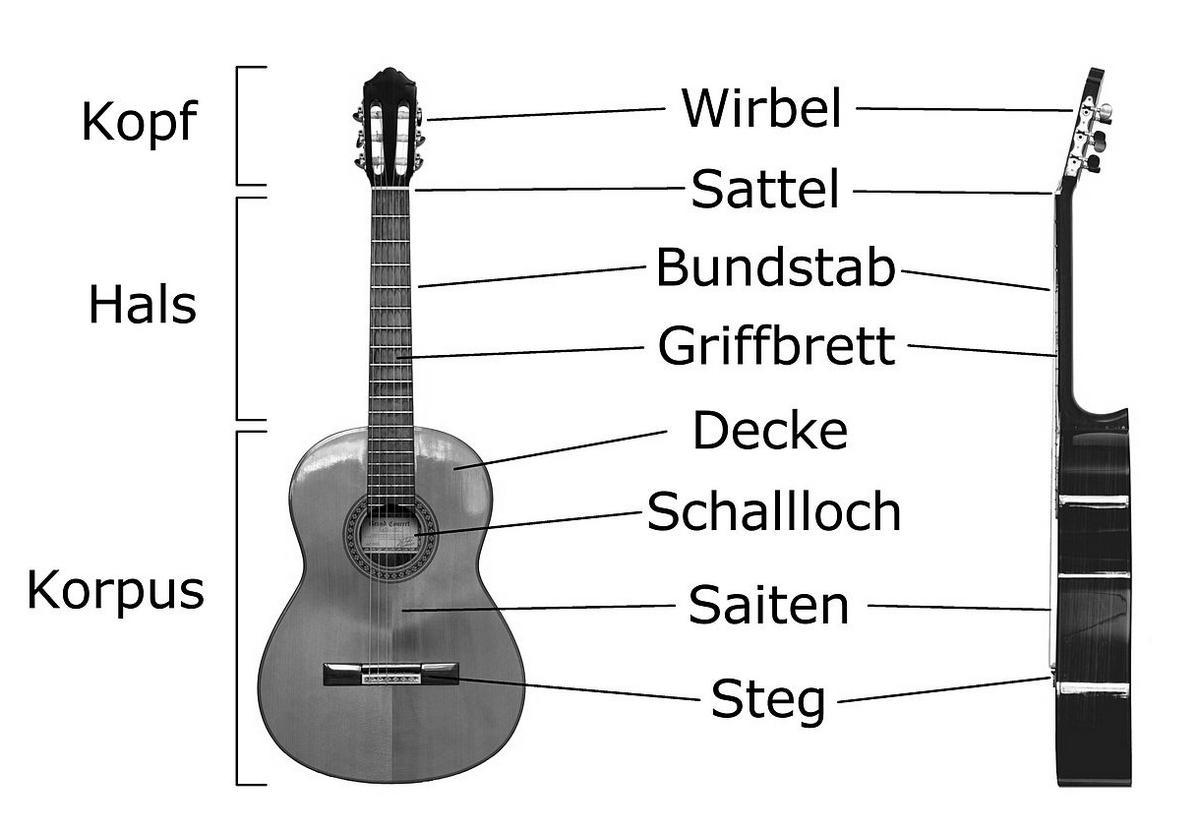
\includegraphics{bilder/gitarre_aufbau.jpg}
	\caption{Aufbau einer Konzertgitarre}
\end{figure}

Am Griffbrett der Gitarre mit den Bundstäbchen kann man Töne abgreifen. Der Abstand zwischen zwei Bundstäbchen ist dabei ein Halbtonschritt. Dadurch können identische Töne auf verschiedenen Saiten gespielt werden.

\begin{table}[H]
\centering
\begin{tabular}{c|cccccc}
Saite & 1 & 2 & 3 & 4 & 5 & 6 \\
\hline
Note & e' & b & g & d & A & E \\
\hline
Frequenz / Hz & 329.63 & 246.94 & 196.00 & 146.83 & 110.00 & 82.41  
\end{tabular}
\caption{Frequenzen der Leersaiten}
\end{table}

Durch die Überlagerung zweier Schwingungen ähnlicher Frequenz kommt es zu Schwebungseffekten. Dabei ändert sich die Amplitude der resultierenden Schwingung periodisch. Für zwei Schwingungen gleicher Amplitude gilt folgendes Additionstheorem
$$\sin(\omega_1t)+\sin(\omega_2t) = 2\sin\left( \frac{\omega_2+\omega_1}2t \right) \cos\left( \frac{\omega_2-\omega_1}2t \right)$$
Es ergibt sich eine Schwebungsfrequenz $\omega_S$ und eine resultierende Frequenz $\omega_R$ gemäß
$$\omega_S = \frac{\omega_2-\omega_1}2 \hspace{0.5cm} \text{ und } \hspace{0.5cm} \omega_R = \frac{\omega_2+\omega_1}2.$$
Dieses Phänomen wird im ersten Teilexperiment untersucht.
Beim Anschlagen einer Gitarrensaite breiten sich Transversalwellen in beide Richtungen aus und werden an Steg und Sattel reflektiert. Dadurch bilden sich stehende Wellen auf der Saite aus. 

\begin{figure}[h]
	\centering
	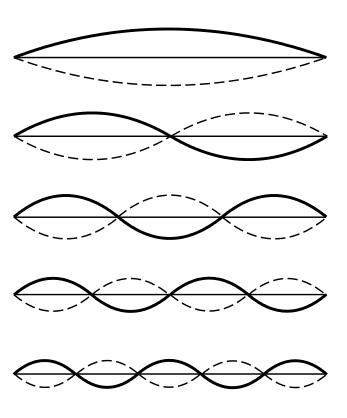
\includegraphics{bilder/StehendeWelle.jpg}
	\caption{Stehende Welle und deren Harmonische bis $n=5$}
\end{figure}

Da die Stehenden Wellen an den Enden der Saite jeweils Knoten ausbilden, gilt für die Wellenlängen der Moden
$$\lambda_n = \frac{2L}n$$
mit $n\in \mathbb N$ und $L$ als Saitenlänge. Die Auslenkung der Saite ergibt sich dabei als Summe der Moden
$$y(x,t) = \sum_{n=1}^\infty A_n \cos(\omega_nt + \phi_n)\sin(k_nx)$$
mit $k_n = \frac{2\pi}{\lambda_n}$. Der Anschlagpunkt der Saite ist entscheidend für das Auftreten der Moden. Schlägt man die Saite im Abstand $d=\frac Ln$ an, so fehlt die $n$-te Harmonische und ihre Vielfachen. Dies wird im zweiten Teilexperiment untersucht.


\subsection{Versuchsaufbau}

\begin{figure}[h]
	\centering
	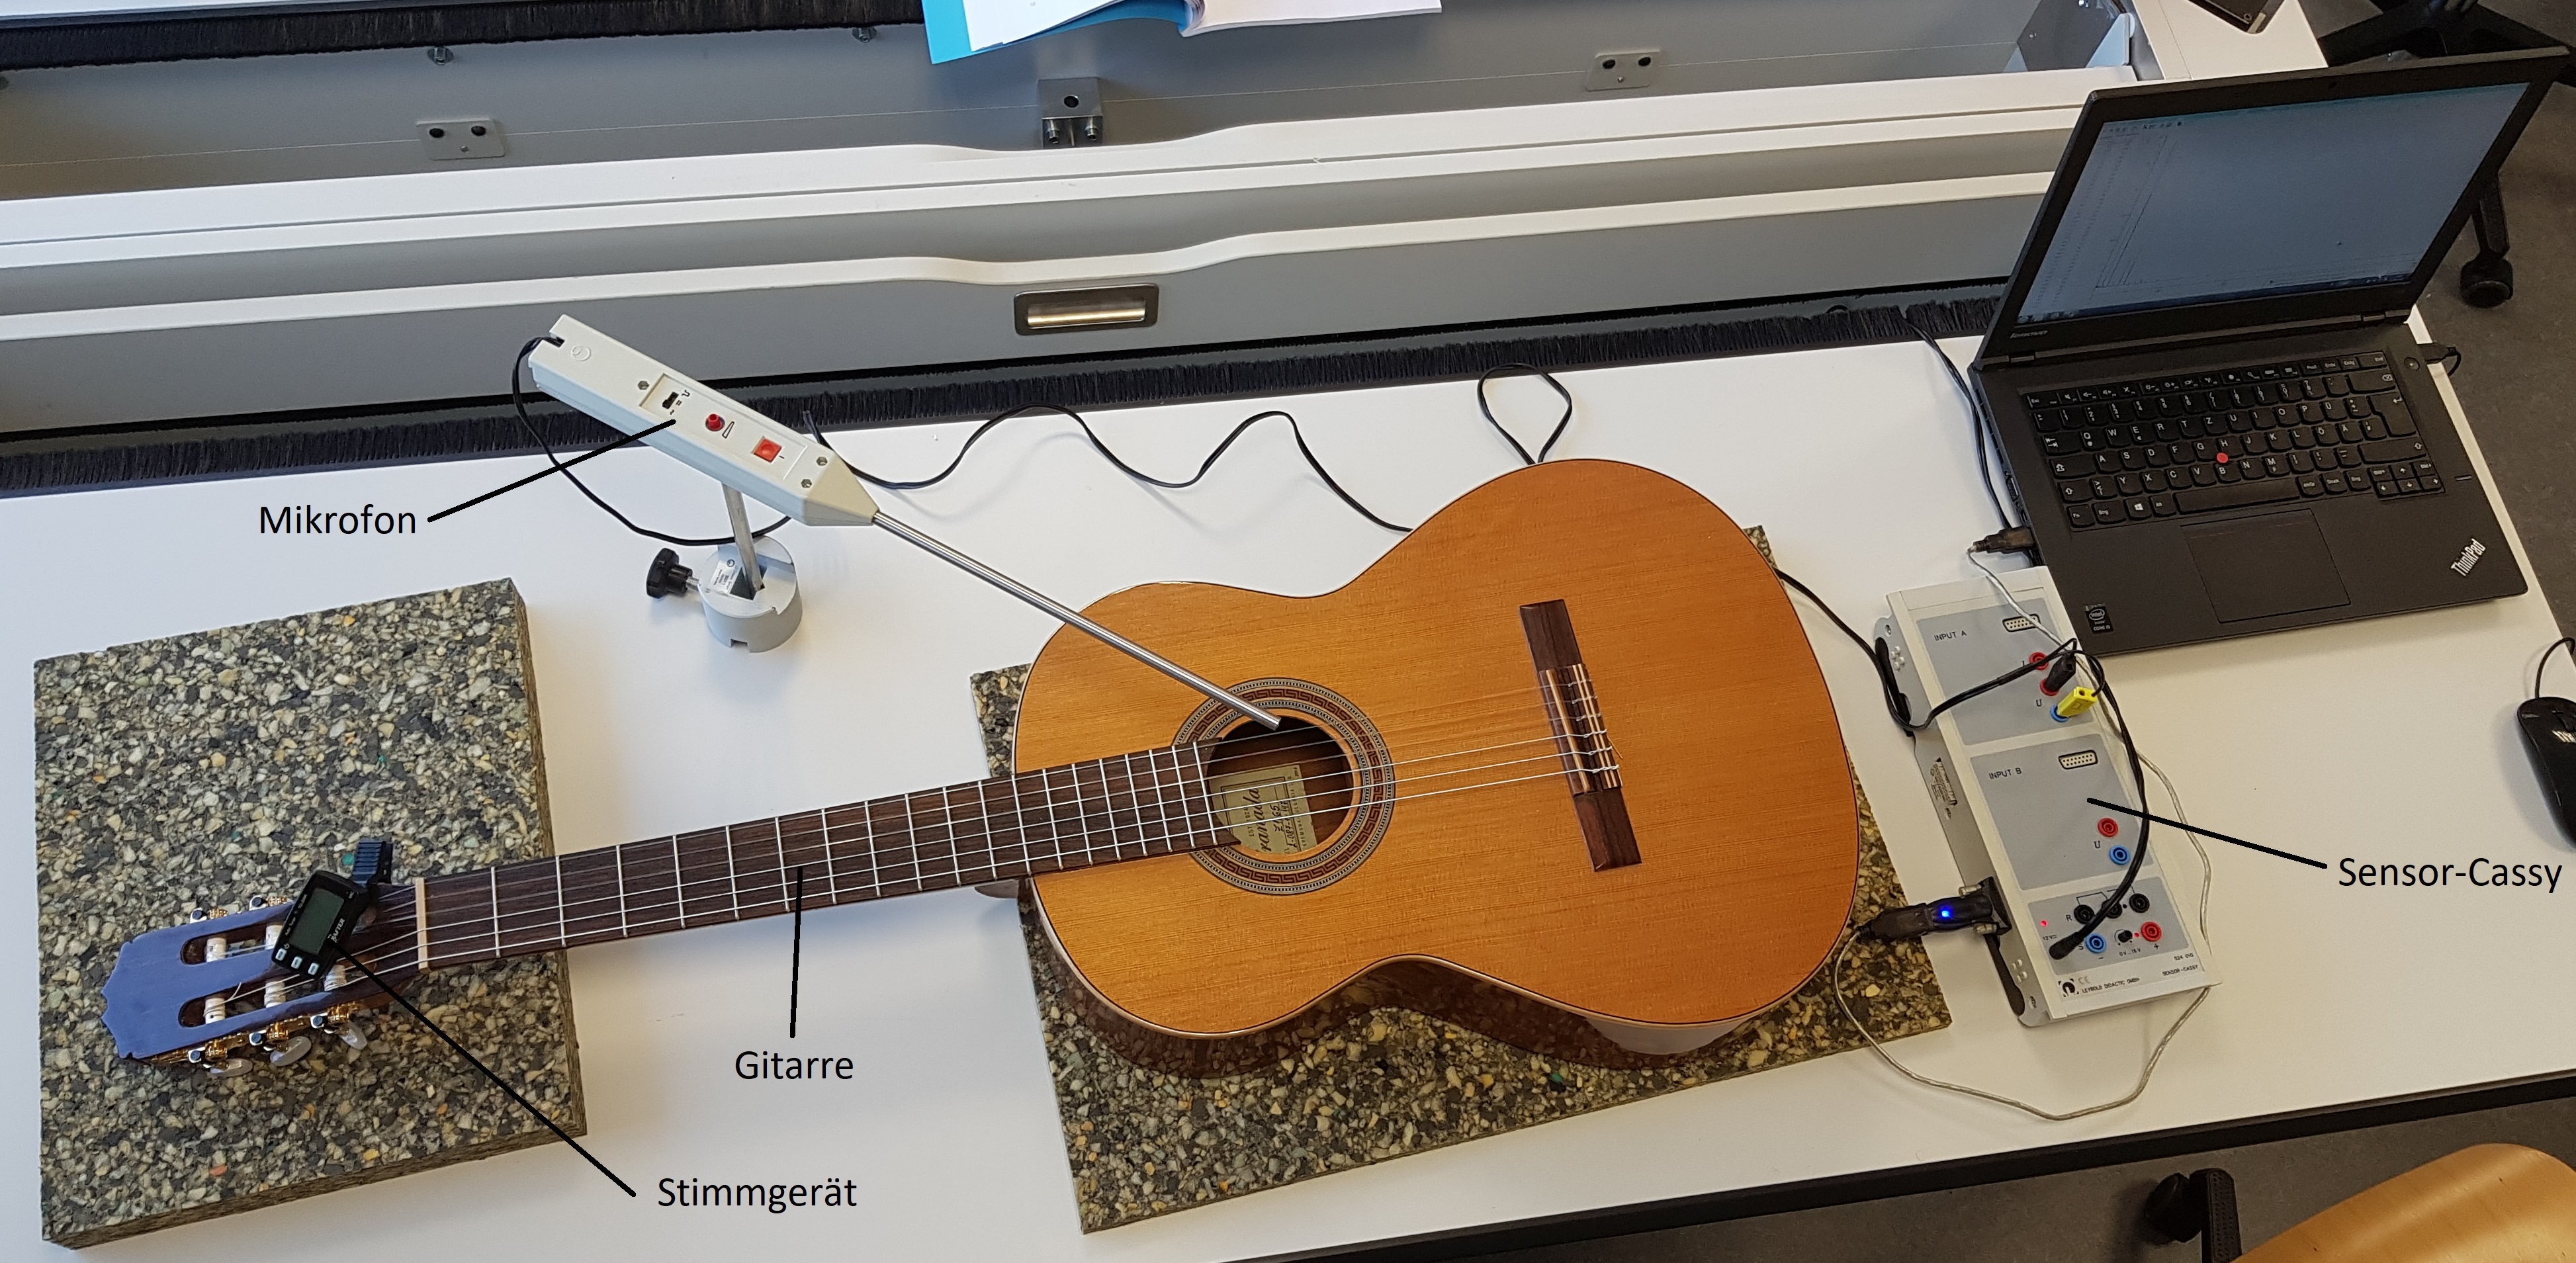
\includegraphics[width=\linewidth]{bilder/gitarre_beschriftet.jpg}
	\caption{Versuchsaufbau}
	\label{aufbauGitarreExp}
\end{figure}

Eine Akustikgitarre liegt auf einer Polsterung auf dem Tisch. Das Mirkofon wird mit einem Stativ mittig oberhalb des Schallochs der Gitarre platziert. Das Mikrofon wird im Amplitudenmodus betrieben und mit dem Sensor-CASSY wird die Ausgangsspannung des Mirkofons gemesssen (vgl. Abb. \ref{aufbauGitarreExp}). Vor der Messung wird die Gitarre mit einem Stimmgerät mit Stimmgenauigkeit von $\pm 1 \, \mathrm{Cent}$ gestimmt.


\subsection{Messung der Schwebung}


\subsubsection{Versuchsdurchführung}

Nach dem Stimmen der Gitarre wird die A-Saite leicht verstimmt. Anschließend wird die offene D-Saite zusammen mit der im 5. Bund gegriffenen A-Saite angeschlagen und eine Messung mit dem Mikrofon gestartet. Es werden für vier verschiedene Verstimmungen Messungen aufgenommen. Dabei wird für die erste Verstimmung eine Messung aufgenommen und für die restlichen drei jeweils zwei Messungen. Für die ersten beiden, sowie die letzte Messung hat das Sensor-CASSY folgende Messparameter:
\begin{enumerate}[-]
\setlength{\itemsep}{-5pt} 
\item Messbereich: $-10$ bis $10\,$V
\item Intervall: $200\,\mu$s
\item Messungen: $16000$
\item Messzeit: $3.2\,$s
\end{enumerate}
Für die anderen Messungen werden folgende Messparameter verwendet:
\begin{enumerate}[-]
\setlength{\itemsep}{-5pt} 
\item Messbereich: $-10$ bis $10\,$V
\item Intervall: $500\,\mu$s
\item Messungen: $16000$
\item Messzeit: $8\,$s
\end{enumerate}


\subsubsection{Versuchsauswertung}

Die Rohdaten der Messung sind exemplarisch in Abbildung \ref{rohSch} zu sehen.

\begin{figure}[h]
	\centering
	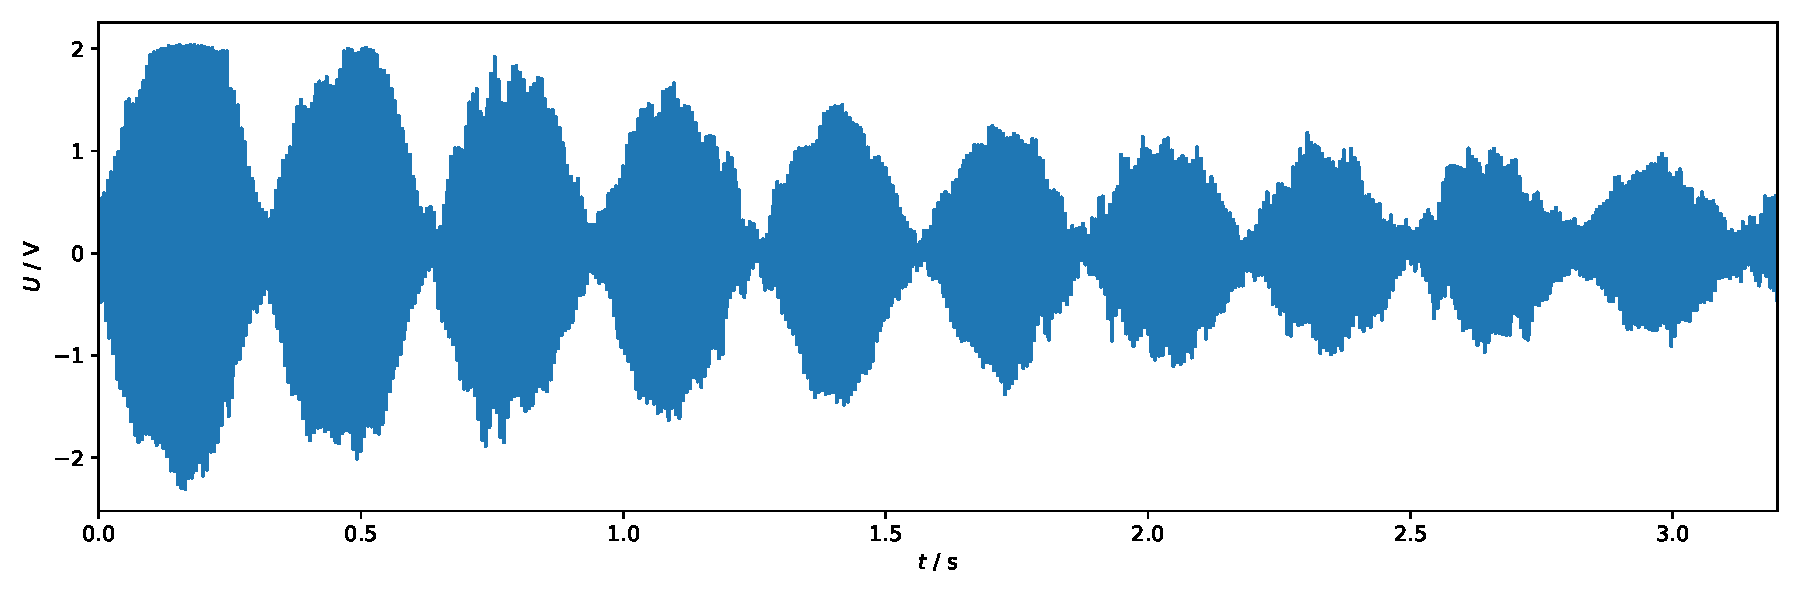
\includegraphics[width=\linewidth]{plots/rohdaten_schwebung.pdf}
	\caption{Visualisierung der Rohdaten aus der ersten Messung (\mbox{``schwebung\_1.lab''})}
	\label{rohSch}
\end{figure}

Wir bestimmen nun die Schwebungsfrequenz $f_S$ und die Frequenz der resultierenden Schwingung $f_R$ auf zwei unterschiedliche Arten. Zum einen durch Ablesen von Maxima/Minima aus den Rohdaten und zum anderen durch eine Fast Fourier Transformation (FFT) der Rohdaten. 
In der ersten Variante werden die Maxima/Minima per Augenmaß aus Plots der Rohdaten abgelesen, wie es in Abbildung \ref{MaxAblesen} zu sehen ist. Um eine Unabhängigkeit der daraus erhaltenen Werte zu erreichen wird aus den Dateien \mbox{``schwebung\_1.lab''}, \mbox{``schwebung\_2.1.lab''}, \mbox{``schwebung\_3.2.lab''} und \mbox{``schwebung\_4.2.lab''} abgelesen und die FFT auf die Daten aus den Dateien \mbox{``schwebung\_1.lab''}, \mbox{``schwebung\_2.2.lab''}, \\
\mbox{``schwebung\_3.1.lab''} und \mbox{``schwebung\_4.1.lab''} angewendet.

\begin{figure}[H]
	\centering
	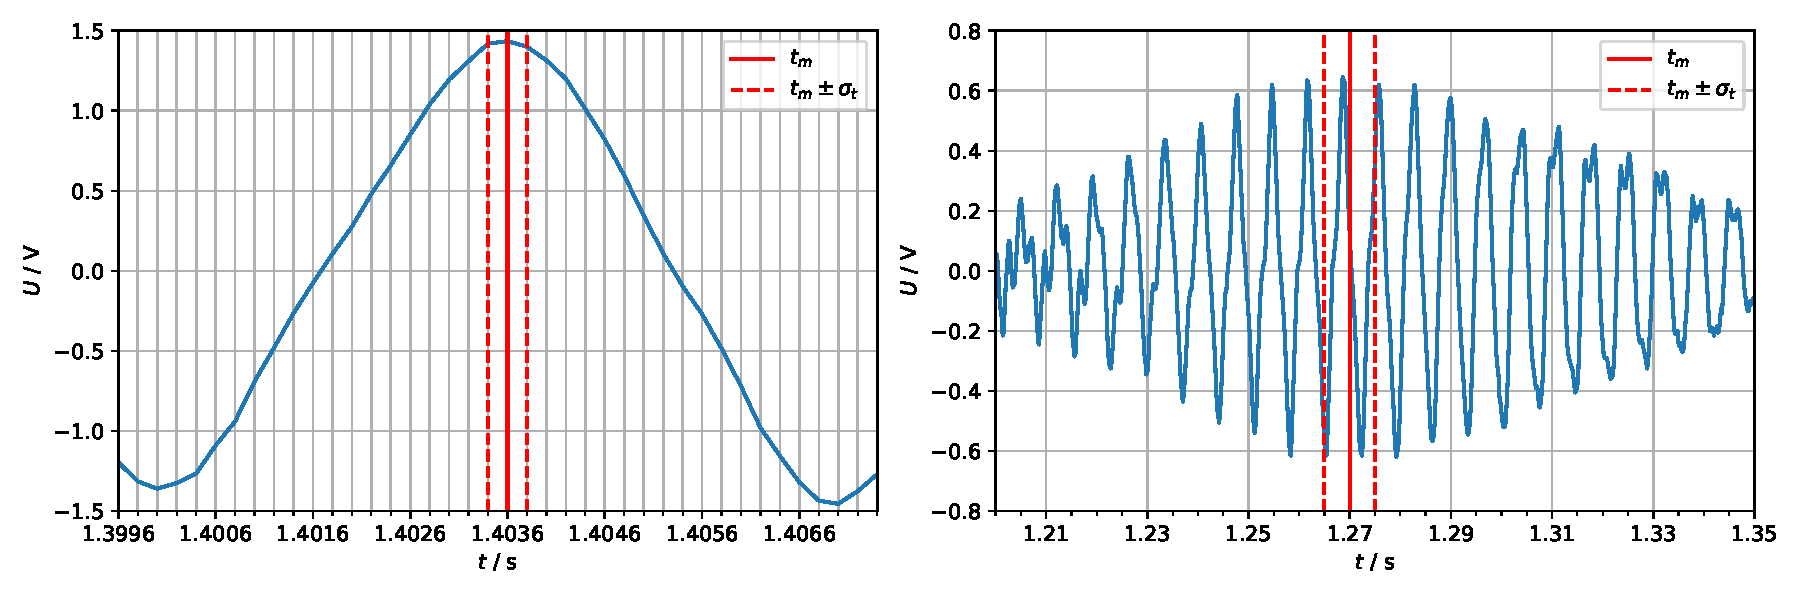
\includegraphics[width=\linewidth]{plots/bspMaxima.pdf}
	\caption{Bestimmung der Maxima aus den Rohdaten}
	\label{MaxAblesen}
\end{figure}
Beim Ablesen für die resultierende Schwingung ist zu beachten, dass sich bei einem Nulldurchgang der Schwebungschwingung die Art das Extremums, welches wir ablesen wollen, ändert. Die so abgelesenen Zeitpunkte sind in Tabelle \ref{tabTimeRes} dokumentiert. Angesichts der Messintervalle für die Zeit und der Erkennbarkeit der Extrema wird für die Schwebungen 1 und 2 die Zeitunsicherheit $\sigma_t = 0.2 \, \mathrm{ms}$, für die Schwebung 3 $\sigma_t = 0.5 \, \mathrm{ms}$ und für die Schwebung 4 $\sigma_t = 0.4 \, \mathrm{ms}$ angesetzt.

\begin{table}[H]
\centering

\begin{adjustbox}{width=\textwidth}
\begin{tabular}{c|c|ccccccccccc}
\multirow{4}{*}{1} 
& $n$ & 1 & 20 & 60 & 80 & 100 & 120 & 140 & 160 & 200 & 236 & 256 \\
\cline{2-13}
& $t$ /s & 0.0308 & 0.1614 & 0.4378 & 0.5754 & 0.7136 & 0.8512 & 0.9892 & 1.1276 & 1.4036 & 1.6518 & 1.7902 \\
\cline{2-13}
& $n$ & 276 & 296 & 336 & 376 & 396 & 416 & 436 & & & & \\
\cline{2-13}
& $t$ / s & 1.9278 & 2.0660 & 2.3418 & 2.6178 & 2.7562 & 2.8936 & 3.0322 & & & & \\
\hline
\multirow{4}{*}{2} 
& $n$ & -2 & 17 & 40 & 60 & 100 & 120 & 140 & 160 & 200 & 220 & 240 \\
\cline{2-13}
& $t$ /s & 0.1548 & 0.2848 & 0.4426 & 0.5802 & 0.8548 & 0.9920 & 1.1292 & 1.2662 & 1.5410 & 1.6782 & 1.8156  \\
\cline{2-13}
& $n$ & 280 & 300 & 320 & 340 & 380 & 400 & 420 & & & & \\
\cline{2-13}
& $t$ / s & 2.0900 & 2.2274 & 2.3648 & 2.5022 & 2.7762 & 2.9136 & 3.0510 & & & &  \\
\hline
\multirow{4}{*}{3}
& $n$ & 6 & 25 & 40 & 60 & 80 & 120 & 140 & 160 & 180 & 200 & 220 \\
\cline{2-13}
& $t$ / s & 0.0070 & 0.1370 & 0.2395 & 0.3765 & 0.5135 & 0.7865 & 0.9235 & 1.0605 & 1.11975 & 1.3345 & 1.4710 \\
\cline{2-13}
& $n$ & 240 & 260 & 280 & 300 & 340 & 360 & 380 & 400 & 420 & 440 & 460 \\
\cline{2-13}
& $t$ /s & 1.6080 & 1.7450 & 1.8820 & 2.0185 & 2.2910 & 2.4285 & 2.5655 & 2.7025 & 2.8395 & 2.9765 & 3.1135 \\
\hline
\multirow{4}{*}{4}
& $n$ & 2 & 20 & 40 & 60 & 80 & 100 & 120 & 180 & 200 & 220 & 240 \\
\cline{2-13}
& $t$ / s & 0.0800 & 0.2060 & 0.3446 & 0.4844 & 0.6234 & 0.7636 & 0.9026 & 1.3214 & 1.4604 & 1.5996 & 1.7388 \\
\cline{2-13}
& $n$ & 280 & 300 & 320 & 340 & 363 & 380 & 400 & 420 & 440 & & \\
\cline{2-13}
& $t$ / s & 2.0188 & 2.1576 & 2.2968 & 2.4366 & 2.5966 & 2.7162 & 2.8552 & 2.9942 & 3.1338 & & 
\end{tabular}
\end{adjustbox}
\caption{Abgelesene Zeitpunkte für die Extrema der resultierenden Schwingung}
\label{tabTimeRes}
\end{table}
Da wir einen linearen Zusammenhang $t(n) = Tn+b$ mit der Periodendauer $T$ für die Zeitpunkte erwarten, führen wir jeweils eine lineare Regression durch. Die Ausgabe der Regressionen ist in Tabelle \ref{tabRegressionRes} abgebildet. 

\begin{table}[H]
\centering
\begin{tabular}{c|c|c|c}
Schwebung & $T$ / ms & $b$ / s & $\chi^2$ / $n_{df}$ \\
\hline
1 & $6.89993 \pm 0.00035$ & $0.02354 \pm 0.00009$ & 1.37 \\
2 & $6.86353 \pm 0.00036$ & $0.16829 \pm 0.00009$ & 0.71 \\
3 & $6.84163 \pm 0.00076$ & $0.0340 \pm 0.0002$ & 0.46 \\
4 & $6.97226 \pm 0.00064$ & $0.0660 \pm 0.0002$ & 0.84
\end{tabular}
\caption{Ergebnisse der Regression für die resultierende Schwingung}
\label{tabRegressionRes}
\end{table}
Das $\chi^2/n_{df}$ von Schwebung 3 deutet auf eine zu grobe Fehlerschätzung hin. Da die Unsicherheit der Zeit in diesem Fall dem Messintervall entspricht, wird an der Unsicherheit festgehalten. Die zugehörigen Residuenplots befinden sich in Abbildung \ref{residuenRes}.


\begin{figure}[H]
	\centering
	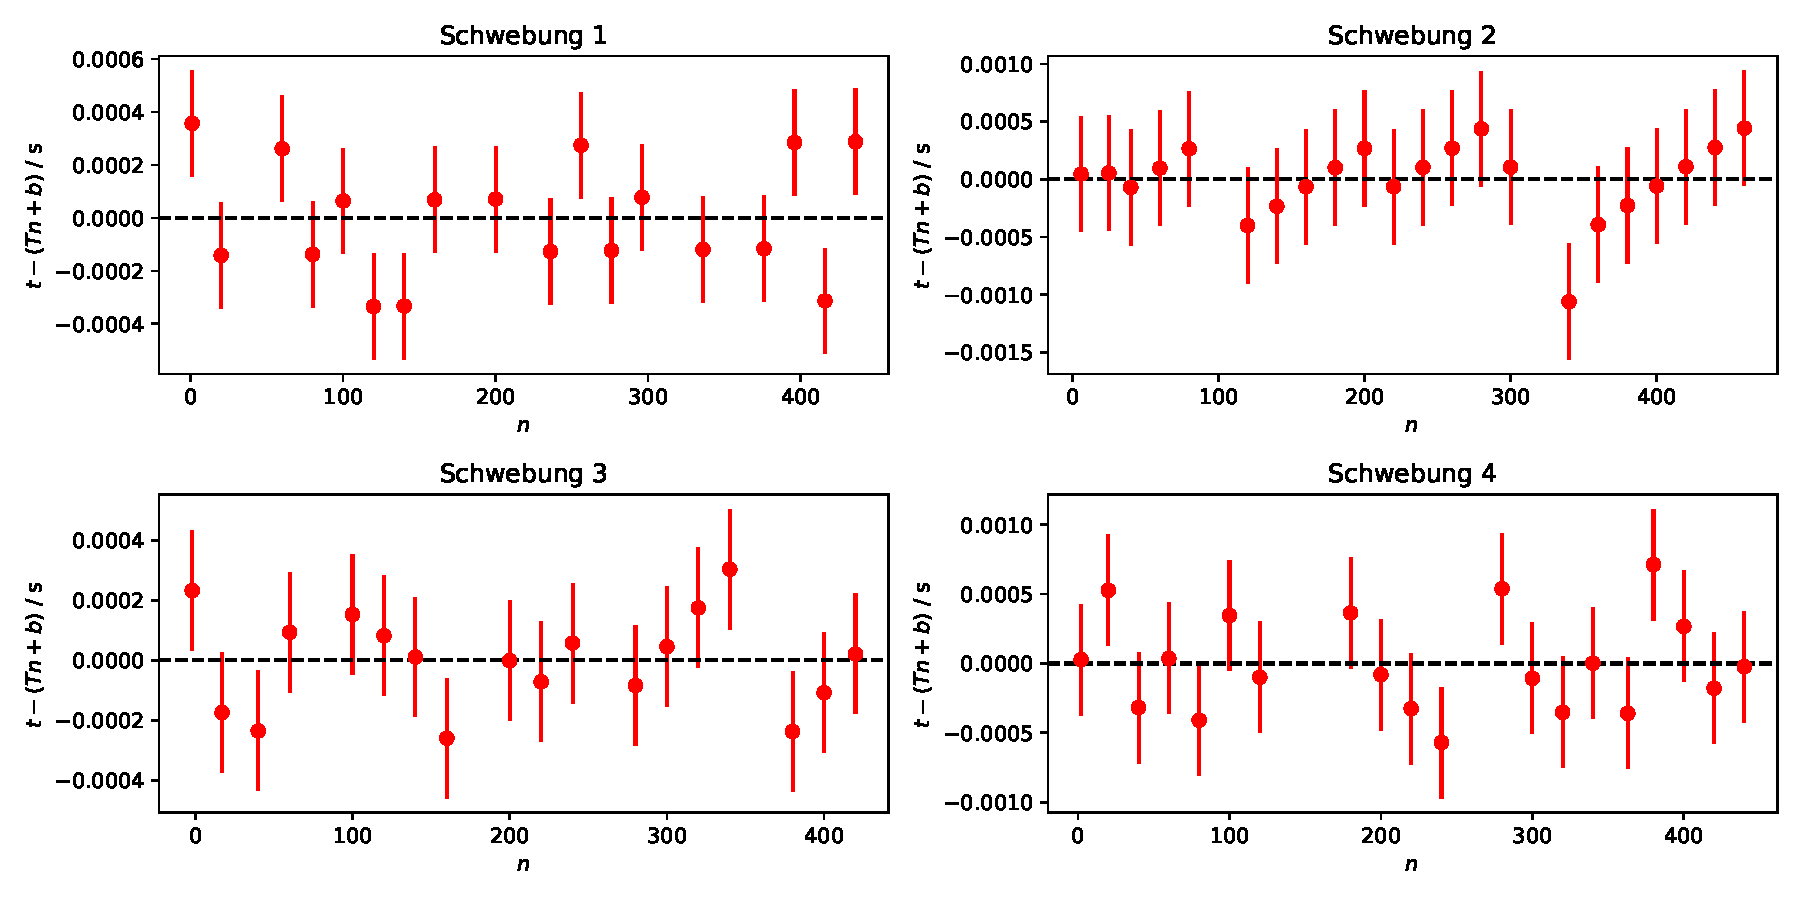
\includegraphics[width=\linewidth]{plots/residuenRes.pdf}
	\caption{Residuenplots der Regression für die resultierende Schwingung}
	\label{residuenRes}
\end{figure}

Bei Schwebung 2 könnte man eine Systematik vermuten. Es wurden jedoch die Abstände der Extrema bei den Sprüngen nochmals nachgeprüft. Nun werden die Zeitpunkte der Extrema der Schwebungsschwingung bestimmt. Die Zeiten sind in Tabelle \ref{tabTimeSch} aufgeführt. Für die Unsicherheiten der Zeitbestimmung wird für die Schwebungen 1 und 4 $\sigma_t = 0.005 \, \mathrm s$ und für die Schwebungen 2 und 3 $\sigma_t = 0.01 \, \mathrm s$ geschätzt.
\begin{table}[H]
\centering
\begin{tabular}{c|c|cccccccccc}
& $m$ & 1 & 2 & 3 & 4 & 5 & 6 & 7 & 8 & 9 & 10 \\
\hline
1 & \multirow{4}{*}{$t$ / s} & 0.155 & 0.465 & 0.780 & 1.085 & 1.410 & 1.720 & 2.035 & 2.345 & 2.655 & 2.975 \\
\cline{1-1}\cline{3-12}
2 & & 0.38 & 1.02 & 1.66 & 2.33 & 2.99 & & & & & \\
\cline{1-1}\cline{3-12}
3 & & 1.30 & 2.82 & & & & & & & & \\
\cline{1-1}\cline{3-12}
\multirow{3}{*}{4}
& & 0.075 & 0.240 & 0.420 & 0.595 & 0.760 & 0.930 & 1.100 & 1.270 & 1.445 & 1.620 \\
\cline{2-12}
& $m$ & 11 & 12 & 13 & 14 & 15 & 16 & 17 & 18 & & \\
\cline{2-12}
& $t$ / s & 1.795 & 1.965 & 2.135 & 2.305 & 2.470 & 2.640 & 2.810 & 2.975 & & 
\end{tabular}
\caption{Abgelesene Zeitpunkte für die Extrema der Schwebungsschwingung}
\label{tabTimeSch}
\end{table}
Wir erwarten wiederum einen linearen Zusammenhang $t(m) = \frac T2m + c$ mit der Periodendauer $T$ der Schwebungschwingung. Wir führen also eine lineare Regression durch mit den Resultaten in Tabelle \ref{tabRegressionSch}.

\begin{table}[H]
\centering
\begin{tabular}{c|c|c|c}
Schwebung & $T$ / ms & c & $\chi^2$ / $n_{df}$ \\
\hline
1 & $ 0.6266 \pm 0.0011$ & $ -0.161 \pm 0.003$ & 0.56 \\
2 & $ 1.3060 \pm 0.0063$ & $ -0.28 \pm 0.01$ & 1.43 \\
4 & $ 0.34211 \pm 0.00045$ & $ -0.094 \pm 0.003$ & 1.02
\end{tabular}
\caption{Ergebnisse der Regression für die Schwebungsschwingung}
\label{tabRegressionSch}
\end{table}
Da wir bei Schwebung 3 nur 2 Extrema vernünftig ablesen konnten, wird hier keine Regression gemacht, sondern die Periodendauer mittels $T = 2(t_2-t_1) = 3.04$ bestimmt. Die Unsicherheit beträgt dabei $\sigma_T = 2\sqrt{2} \sigma_t \approx 0.03$. Für die restlichen Schwebungen sind die Residuengraphen in Abbildung \ref{residuenSch}.

\begin{figure}[H]
	\centering
	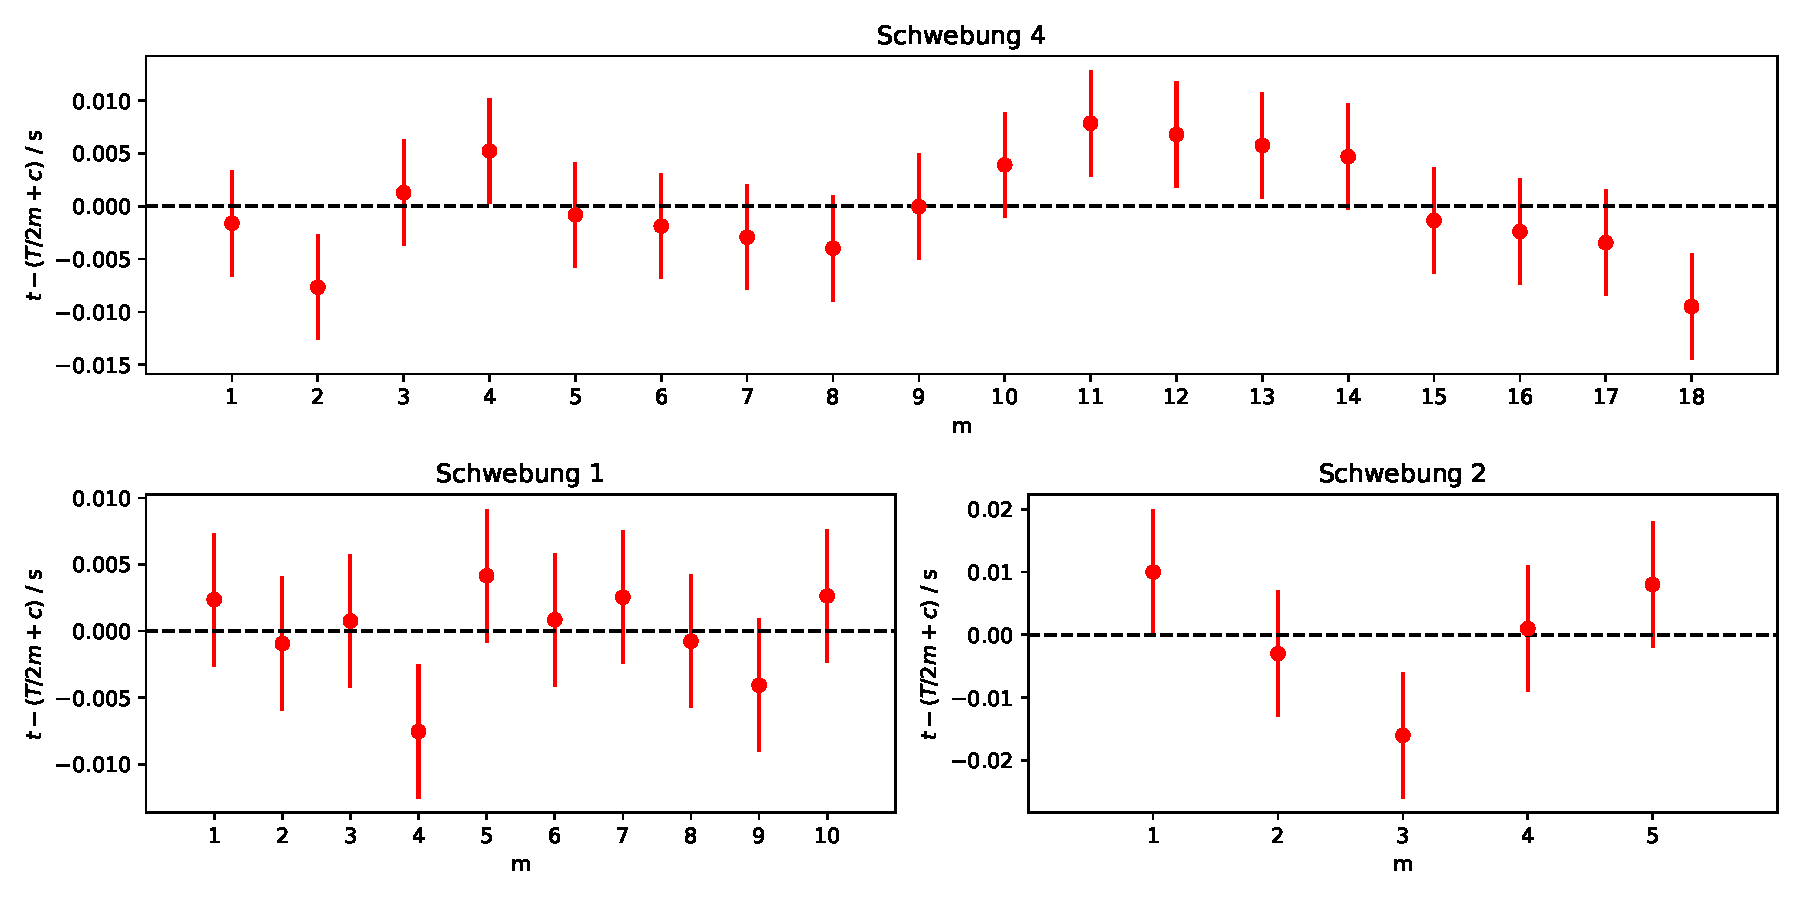
\includegraphics[width=\linewidth]{plots/residuenSch.pdf}
	\caption{Residuenplots der Regression für die Schwebungsschwingung}
	\label{residuenSch}
\end{figure}

Auf den ersten Blick sehen diese gut aus und es lässt sich keine Systematik erkennen.


Nun wollen wir uns dem Frequenzspektrum aus der FFT widmen. In Abbildung \ref{freqSpecSch} ist beispielhaft das Spektrum einer Schwebung abgebildet. Man sieht deutlich zwei Peaks bei etwa 145 Hz. Diese setzen sich zudem kleiner werdend bei den Vielfachen dieser Frequenz fort.
\begin{figure}[H]
	\centering
	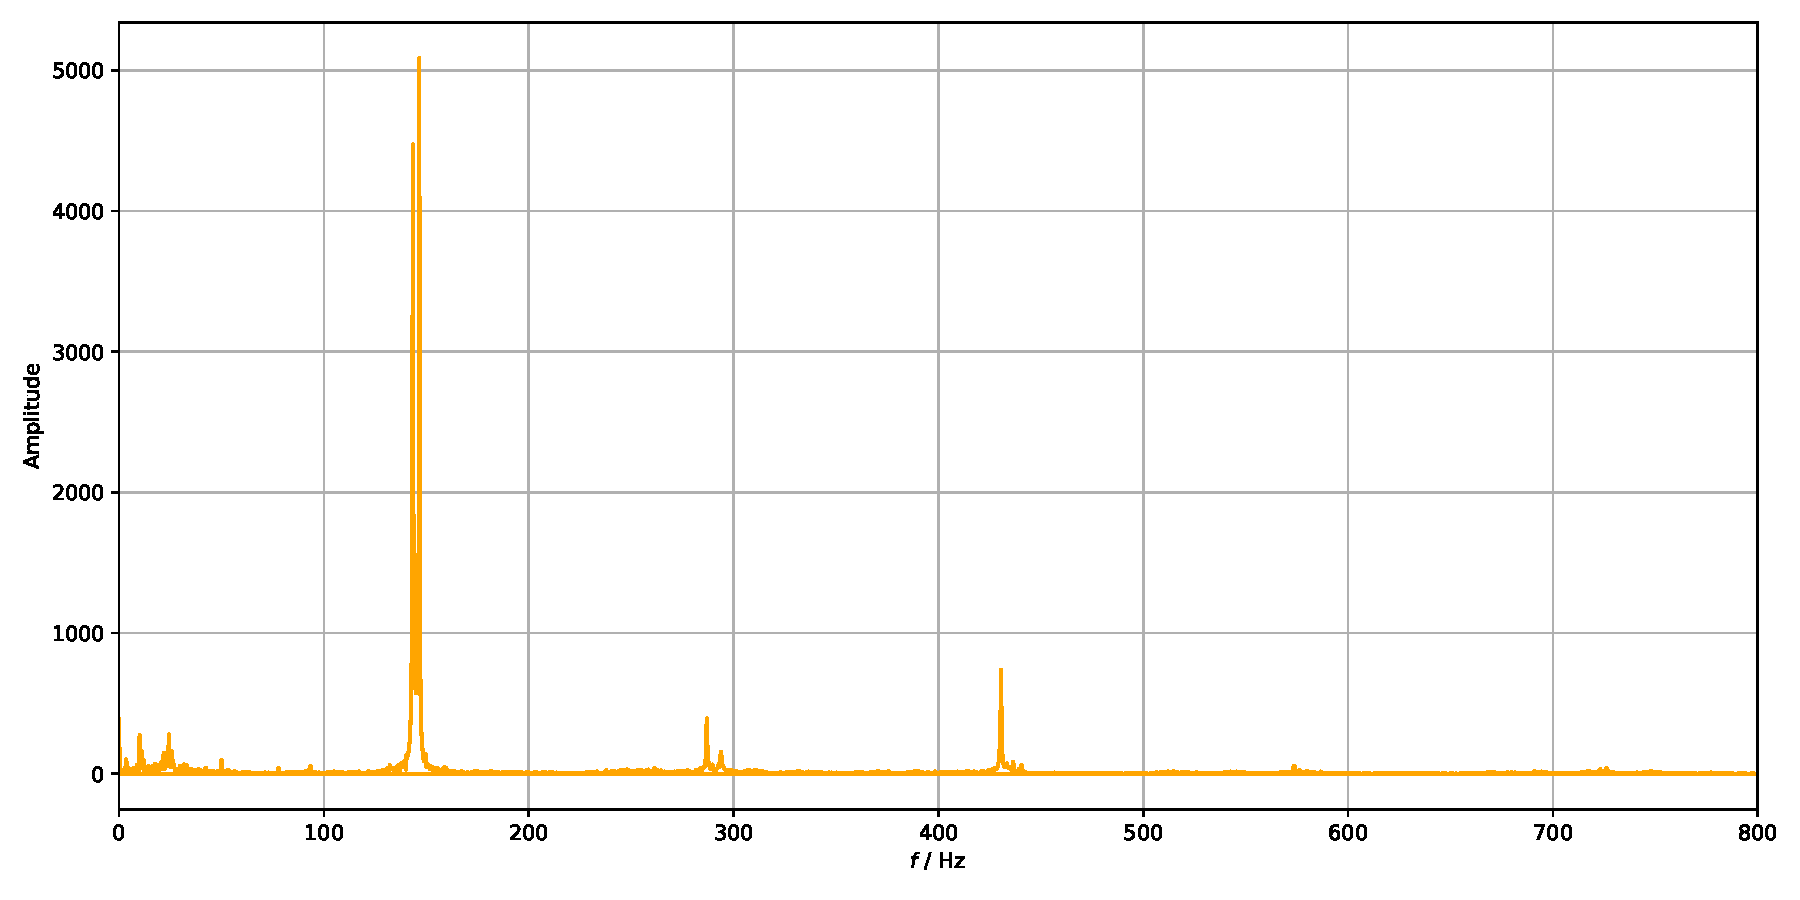
\includegraphics[width=\linewidth]{plots/schwebungsspektrum.pdf}
	\caption{Frequenzspektrum der ersten Messung (\mbox{``schwebung\_1.lab''})}
	\label{freqSpecSch}
\end{figure}

Wir benutzen nun die Peakfinder-Methode der Praktikumsbibliothek um die Frequenzen der Peaks zu bestimmen. Die Resultate sind in Abbildung \ref{fftPeakSch} für alle vier Schwebungen zu sehen.

\begin{figure}[H]
	\centering
	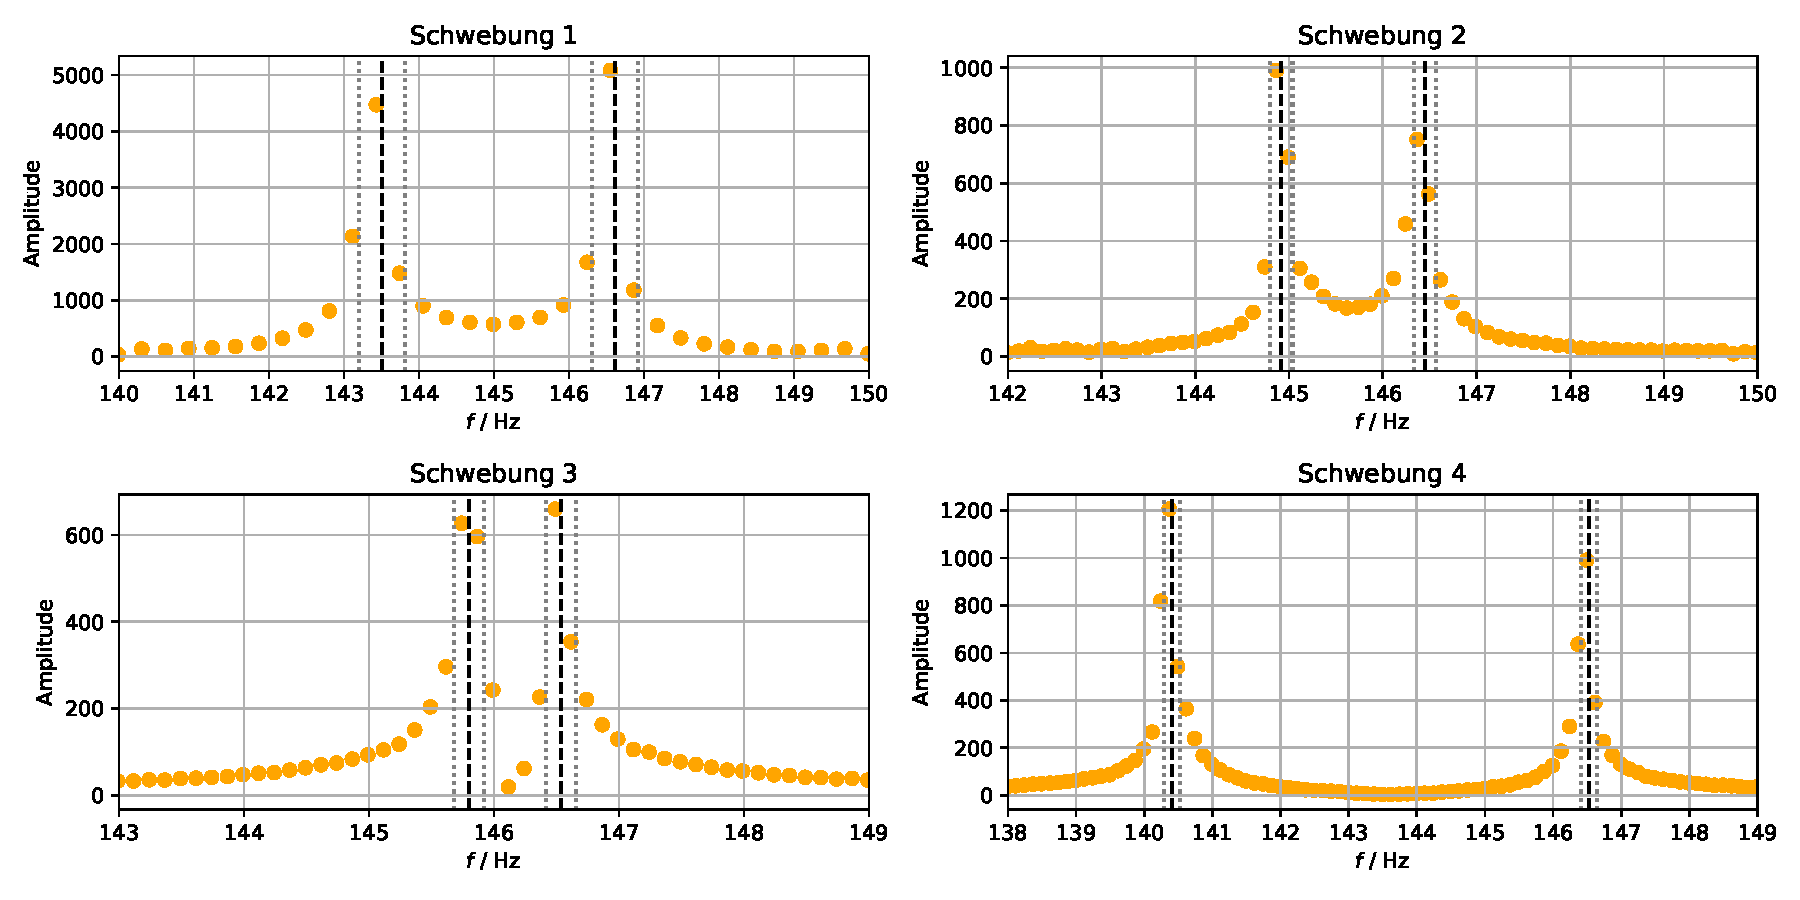
\includegraphics[width=\linewidth]{plots/FFT_freq.pdf}
	\caption{FFT der Schwebungen mit Peakanalyse}
	\label{fftPeakSch}
\end{figure}
Als Fehler wird dabei die Frequenzdifferenz zwischen zwei Punkten in der FFT genommen. Die Ergebnisse der Berechnungen sind in Tabelle \ref{tabFFTpeakSch} aufgelistet. Zudem ist dort auch angegeben auf welche Frequenzbereiche des Spektrums die Peakfinder-Methode angewendet wurde.

\begin{table}[H]
\centering
\begin{tabular}{c|c|c|c|c}
Schwebung & $f_1$ / Hz & Bereich für $f_1$ / Hz & $f_2$ / Hz & Bereich für $f_2$ / Hz \\
\hline
1 & $ 143.51 \pm 0.31$ & 142-145 & $ 146.61 \pm 0.31$ & 145-148 \\
2 & $ 144.92 \pm 0.12$ & 144-145.5 & $ 146.45 \pm 0.12$ & 145.5-147.5 \\
3 & $ 145.85 \pm 0.12$ & 144-146.2 & $ 146.47 \pm 0.12$ & 146.1-148 \\
4 & $ 140.40 \pm 0.12$ & 138-143.5 & $ 146.53 \pm 0.12$ & 143.5-149 
\end{tabular}
\caption{Ergebnisse der Peakanalyse der Frequenspektren}
\label{tabFFTpeakSch}
\end{table}
Mit diesen Werten lassen sich nun die Frequenz der resultierenden Schwingung und der Schwebungsschwingung berechnen, wenn man
$$f_S = \frac{f_2-f_1}2 \, , \hspace{1cm} f_R = \frac{f_2+f_1}2$$
benutzt. Berechnet man zusätzlich anhand der abgelesenen Periodendauern die Frequenzen mittels $f = \frac 1T$, so ergibt sich das Resultat in Tabelle \ref{tabFreqErg}.


\begin{table}[H]
\centering
\begin{tabular}{c|c|c|c|c}
& \multicolumn{2}{c|}{Abgelesen} & \multicolumn{2}{c}{FFT} \\
\hline
Schwebung & $f_S$ / Hz & $f_R$ / Hz & $f_S$ / Hz & $f_R$ / Hz \\
\hline
1 & $ 1.5959 \pm 0.0028$ & $ 144.9290 \pm 0.0074$ & $ 1.55 \pm 0.22$ & $ 145.06 \pm 0.22$ \\
2 & $ 0.7657 \pm 0.0037$ & $ 145.6978 \pm 0.0076$ & $ 0.77 \pm 0.08$ & $ 145.69 \pm 0.08$ \\
3 & $ 0.3289 \pm 0.0032$ & $ 146.164 \pm 0.016$ & $ 0.31 \pm 0.08$ & $ 146.16 \pm 0.08$ \\
4 & $ 2.9230 \pm 0.0038$ & $ 143.426 \pm 0.013$ & $ 3.07 \pm 0.08$ & $ 143.47 \pm 0.08$ 
\end{tabular}
\caption{Ergebnisse der Frequenzen von resultierender und Schwebungs-Schwingung}
\label{tabFreqErg}
\end{table}



\subsubsection{Fazit}

Wir haben nun auf zwei verschiedene Arten Werte für die Frequenzen der Schwebungschwingung und der resultierenden Schwingung erhalten. Zum Vergleich der Werte berechnen wir die relativen Abweichungen.

\begin{table}[H]
\centering
\begin{tabular}{c|c|c|c|c|c|c|c|c}
& \multicolumn{4}{c|}{$f_S$} & \multicolumn{4}{c}{$f_R$} \\
\hline
Schwebung & 1 & 2 & 3 & 4 & 1 & 2 & 3 & 4 \\
\hline
$\frac{|f_1-f_2|}{\sqrt{\sigma_1^2+\sigma_2^2}}$ & 0.21 & 0.05 & 0.24 & 1.84 & 0.60 & 0.10 & 0.05 & 0.54 
\end{tabular}
\end{table}
Die Werte stimmen überwiegend gut überein. Bei Schwebung 4 liegen die Schwebungsfrequenzen $f_S$ weiter auseinander. Es könnte der Fehler bei der Auswertung mit der FFT unterschätzt worden. Besonders die Bestimmung des Peaks ist dabei fraglich. Ein Zusammenhang zur Verwendung von verschiedenen Messungen bei der Auswertung kann ausgeschlossen werden, da eine FFT der anderen Messung diegleichen Frequenzen liefert. 


\subsection{Aufnahme eines Frequenzspektrums}

\subsubsection{Versuchsdurchführung}

In diesem Teilversuch wird das Frequenzspektrum der Gitarre in Abhängigkeit des Anschlagpunktes auf der Saite untersucht. Dazu wird die E-Saite an drei verschiedenen Punkten angeschlagen. Die Saite wird dabei bei $d=\frac 12$, $d=\frac 15$ und $d= \frac 13$ der Saitenlänge angeschlagen. Für den ersten und dritten Anschlagpunkt werden zwei Messungen aufgenommen und für den zweiten eine Messung. Die Messparameter des Sensor-CASSY sind dabei, abgesehen vom Messintervall, wie im ersten Teilversuch. Für die erste Messung liegt das Messintervall bei 200 $\mu$s und für die restlichen bei 100 $\mu$s.


\subsubsection{Versuchsauswertung}

Jeweils eines der Freqeunzspektren für jeden Anschlagpunkt $d$ ist in Abbildung \ref{anschlagSpec} geplottet. Man sieht jeweils gut, dass der Peak für die $1/d$-te Harmonische deutlich weniger ausgeprägt ist, als die Peaks der benachbarten Harmonischen. Bei den Vielfachen ist dies auch noch leicht zu erkennnen. Das die Peaks trotzdem vorhanden sind hängt vermutlich mit einem unsauberen Anschlag zusammen. Theoretisch könnte man die Peakhöhen ablesen und durch Überlagerung der Moden mit den entsprechenden Amplituden die ursprüngliche Auslenkung der Saite rekonstruieren. Das Auftreten eines Peaks bei etwa 3800 Hz in allen Spektren kommt sicher nicht von der Gitarre. Allerdings fehlt uns auch eine andere Erklärung desssen.
\begin{figure}[h]
	\centering
	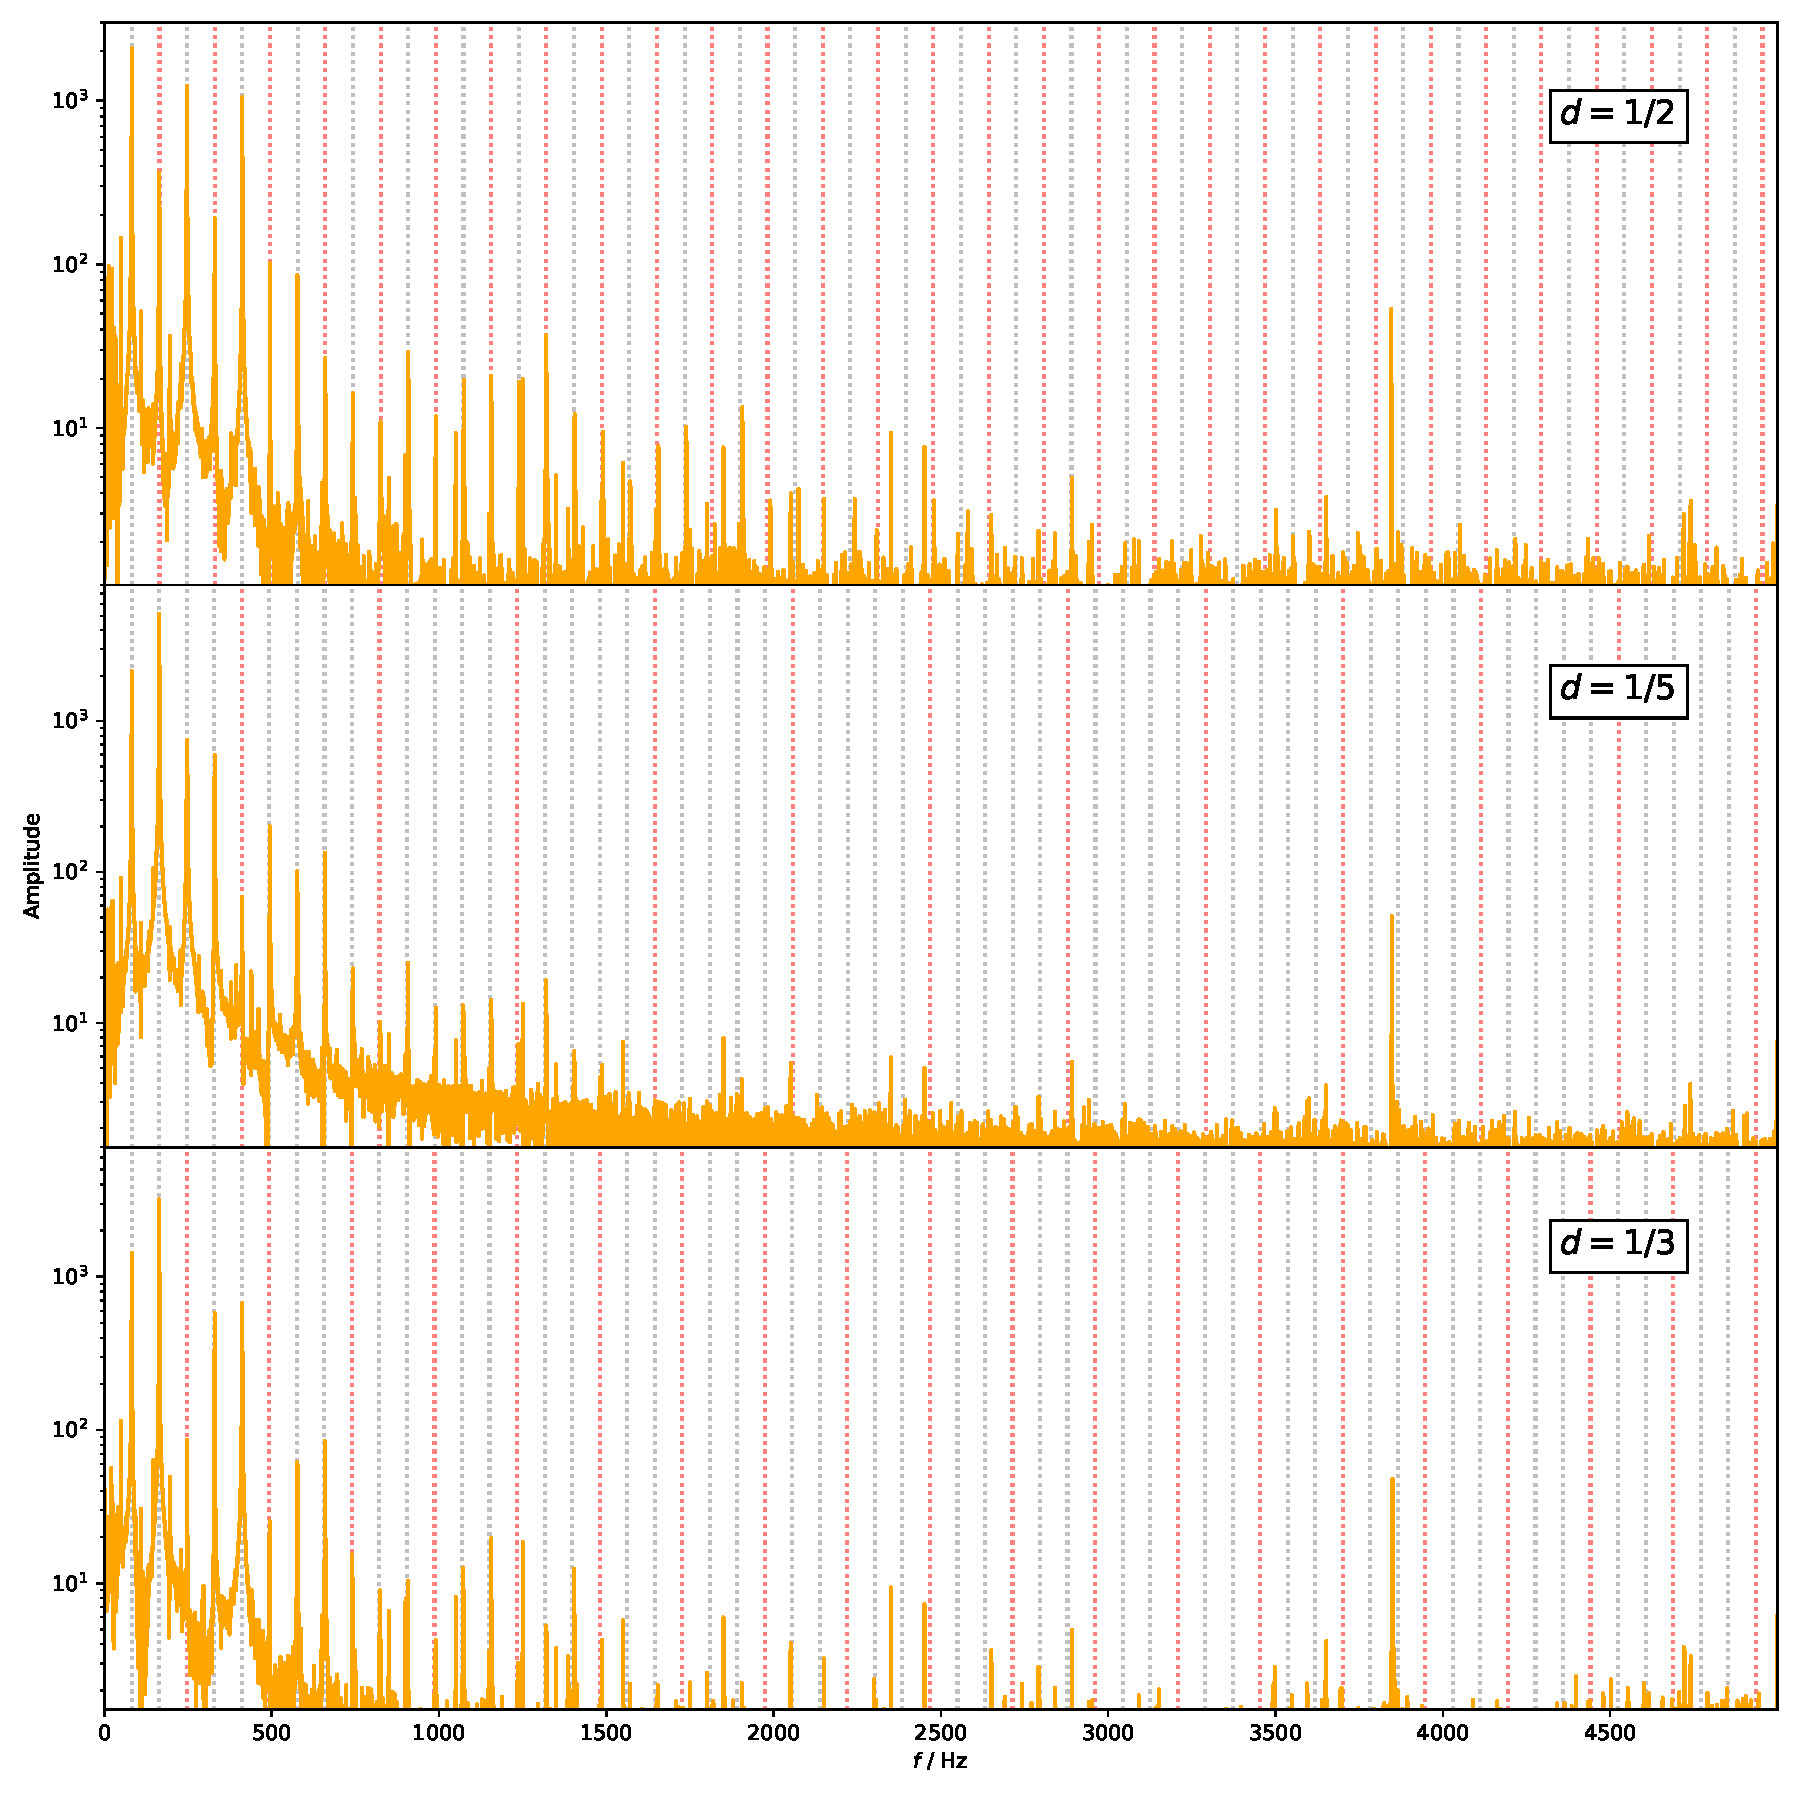
\includegraphics[width=\linewidth]{plots/anschlagspektrum.pdf}
	\caption{Frequenzspektren bei verschiedenen Anschlagpunkten}
	\label{anschlagSpec}
\end{figure}






\nopagebreak
\appendix
\section{Ergebnisse der Peakfinder-Methode}\label{anhang:plot}
\begin{figure}[H]
	\centering
	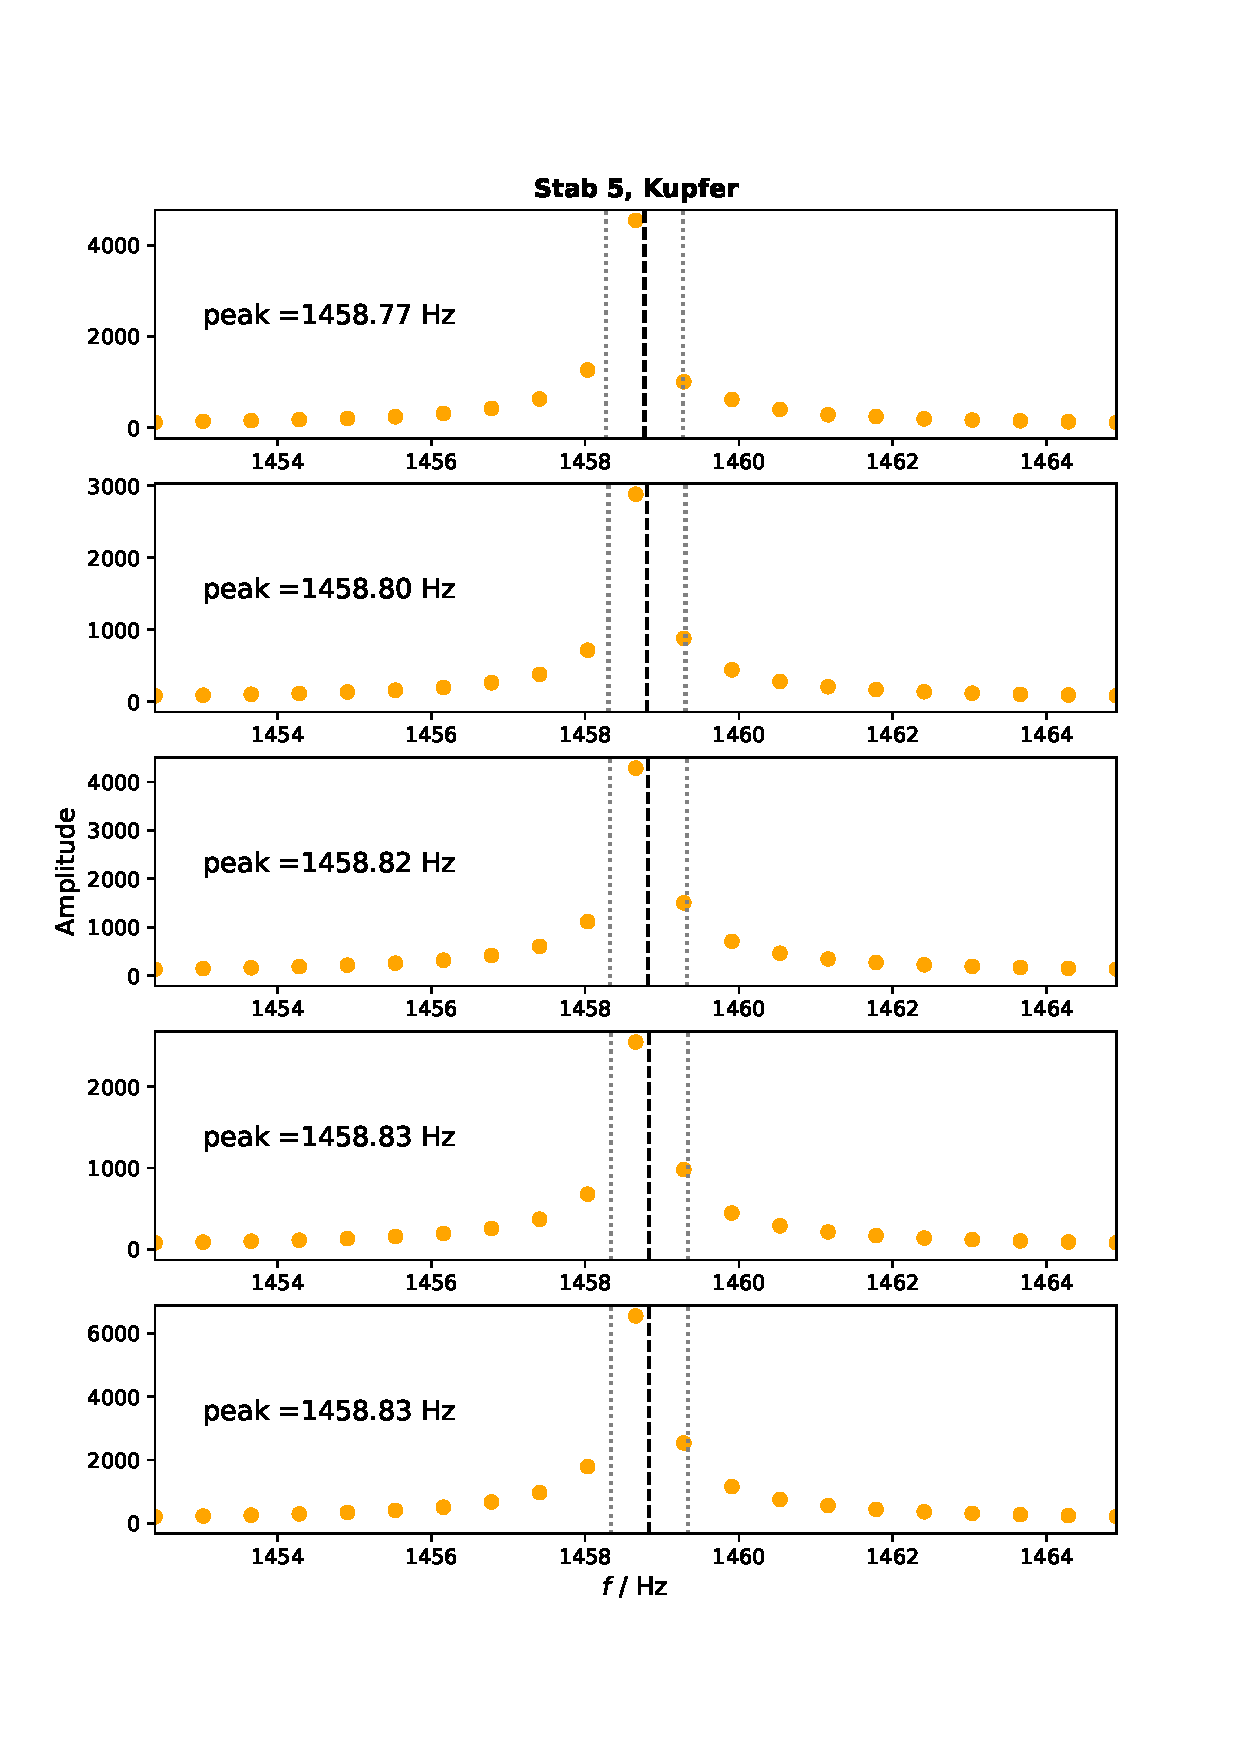
\includegraphics[width=\linewidth]{plots/anhang1.pdf}
\end{figure}

\begin{figure}[H]
	\centering
	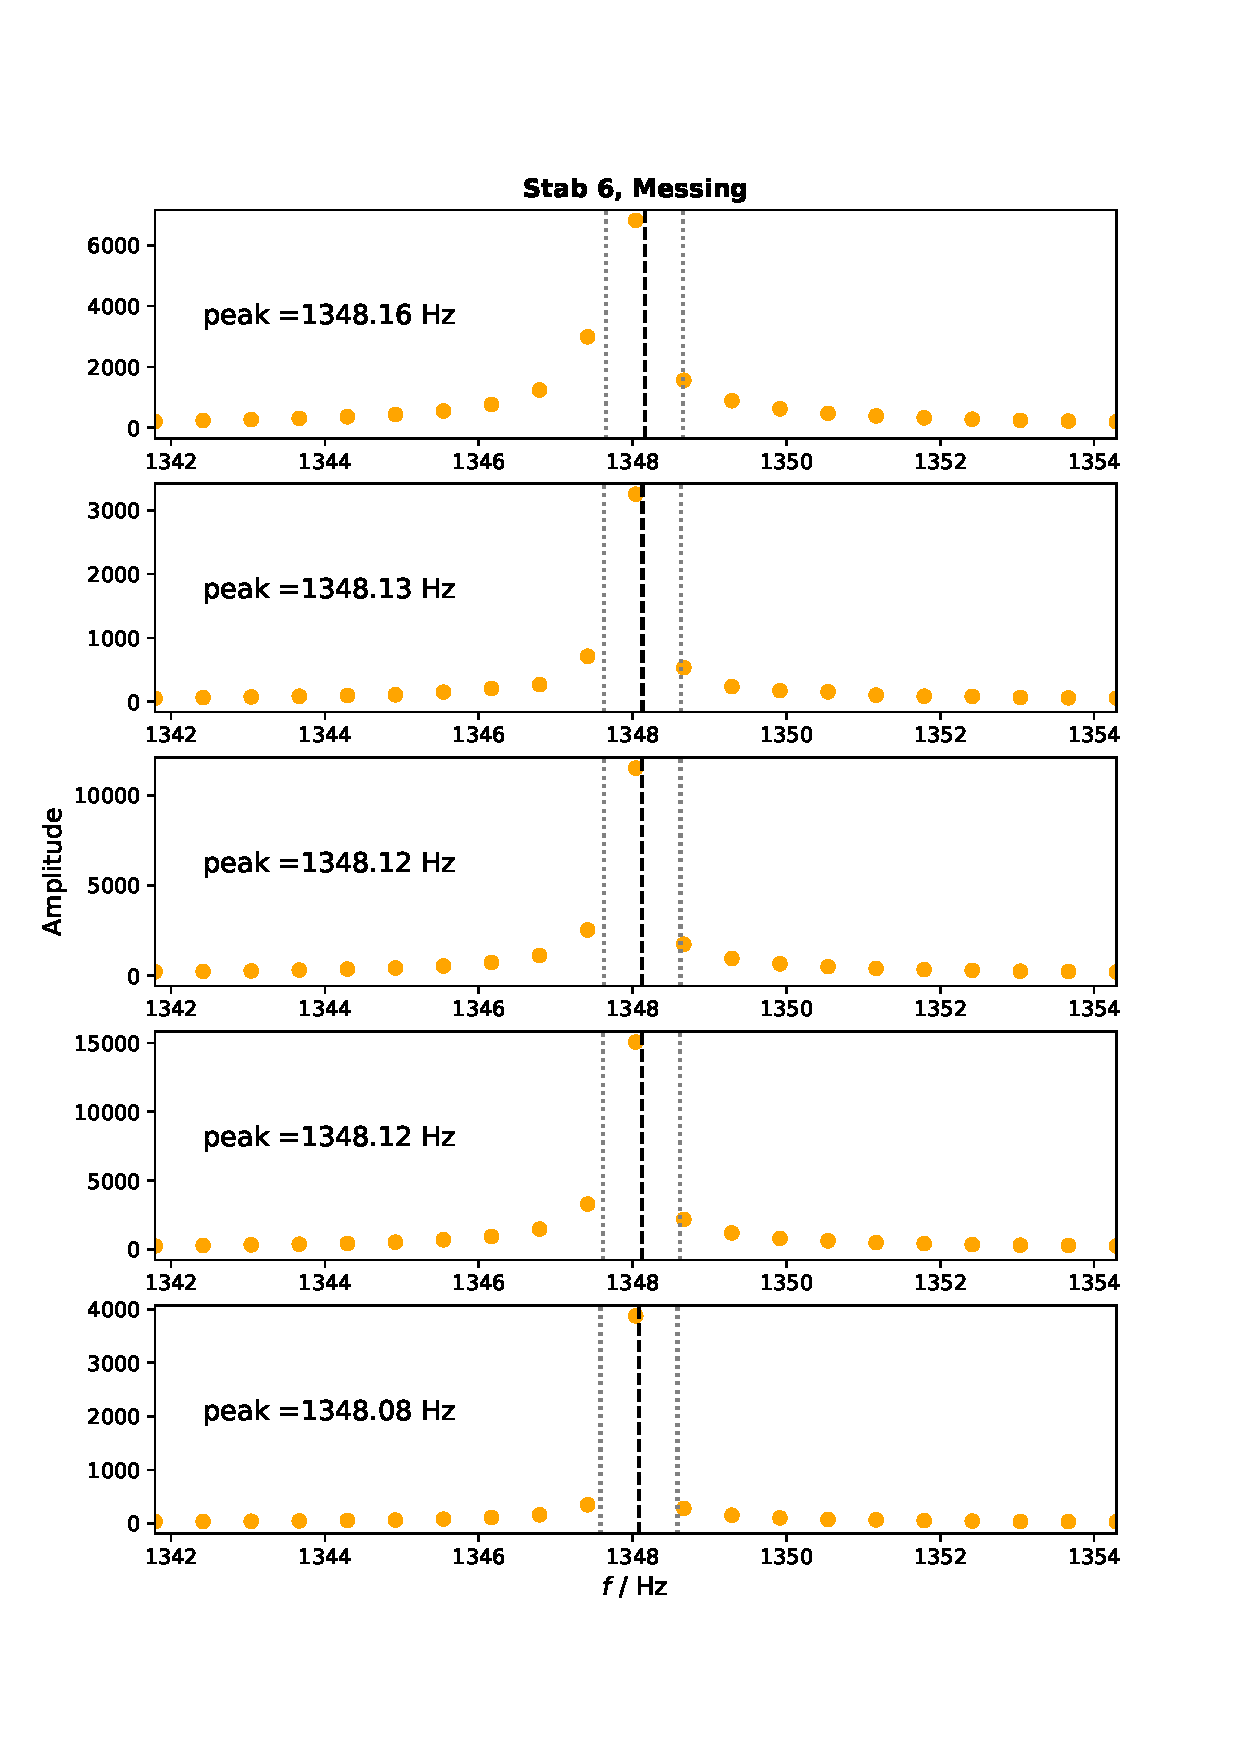
\includegraphics[width=\linewidth]{plots/anhang2.pdf}
\end{figure}

\begin{figure}[H]
	\centering
	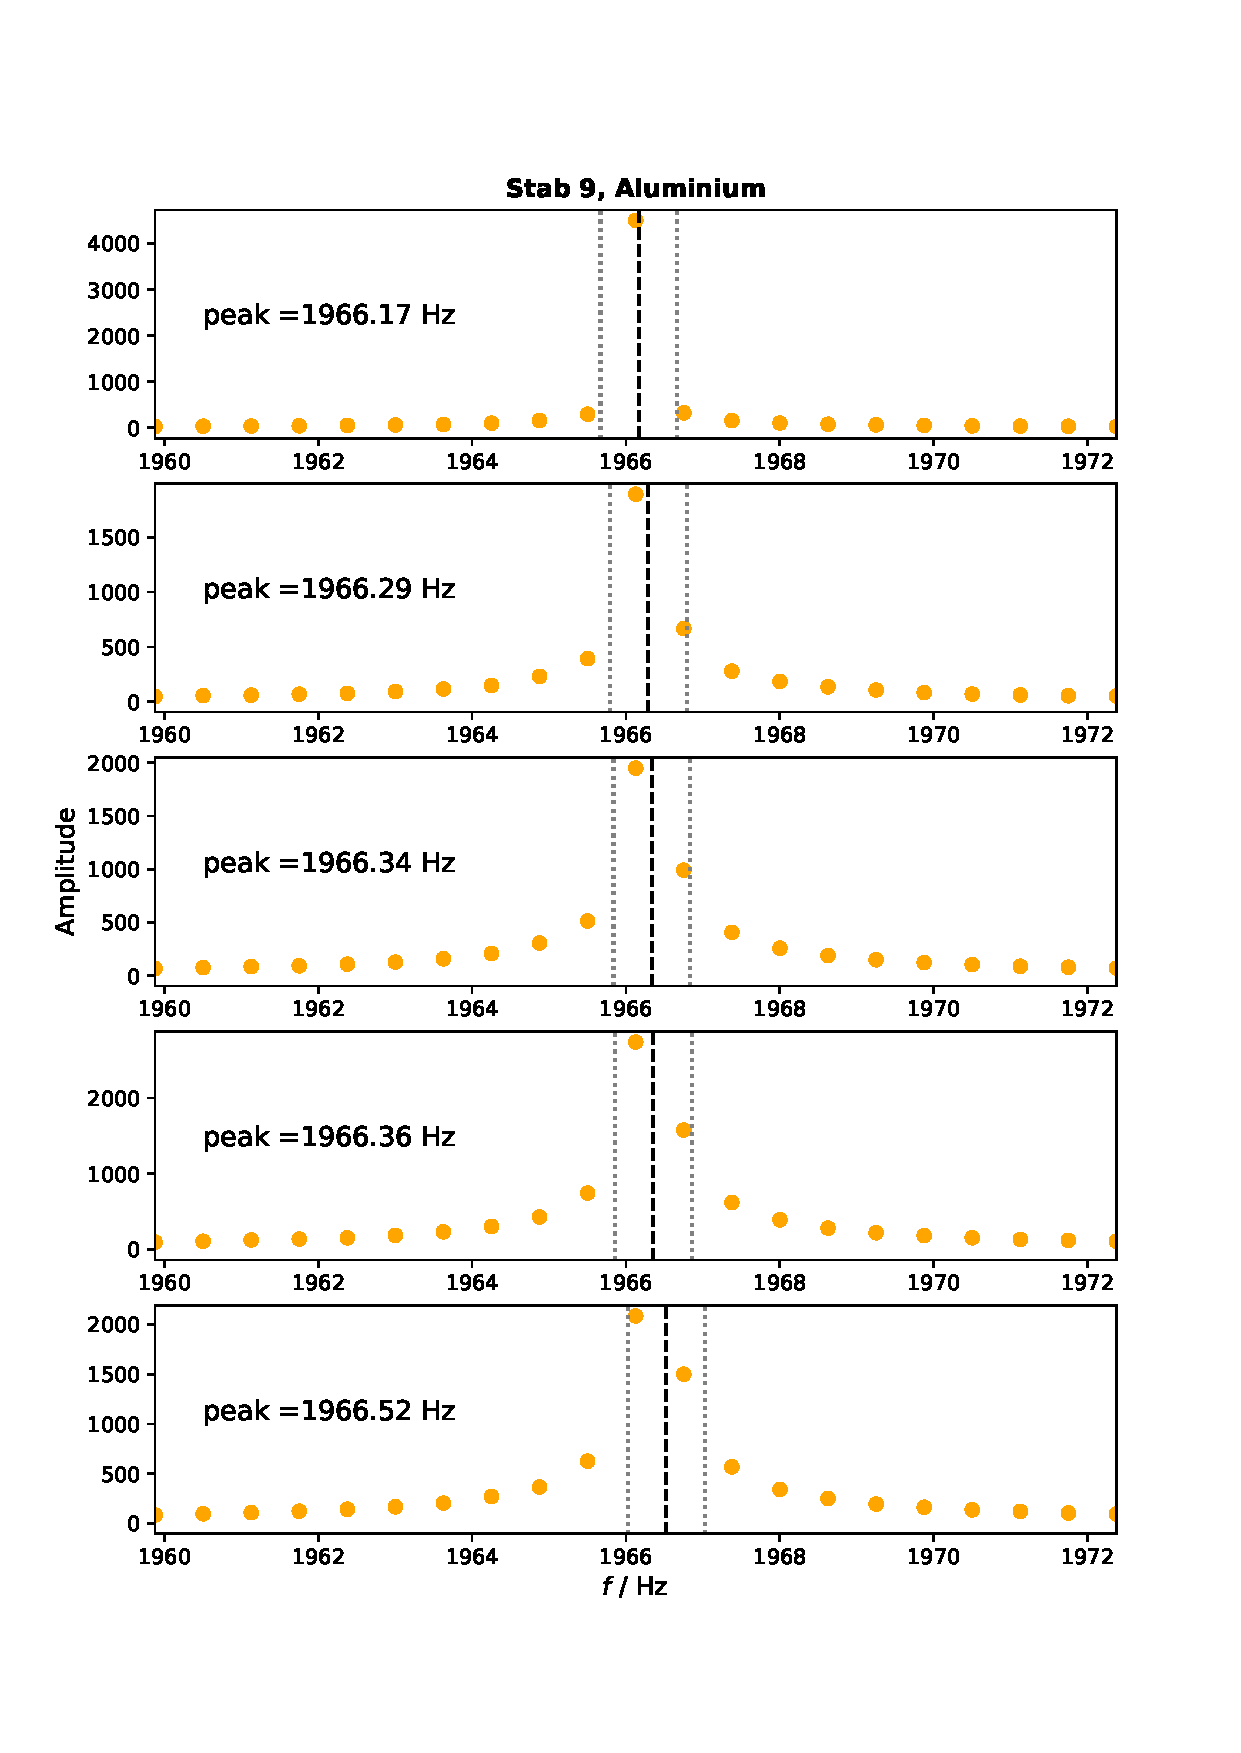
\includegraphics[width=\linewidth]{plots/anhang3.pdf}
\end{figure}

\begin{figure}[H]
	\centering
	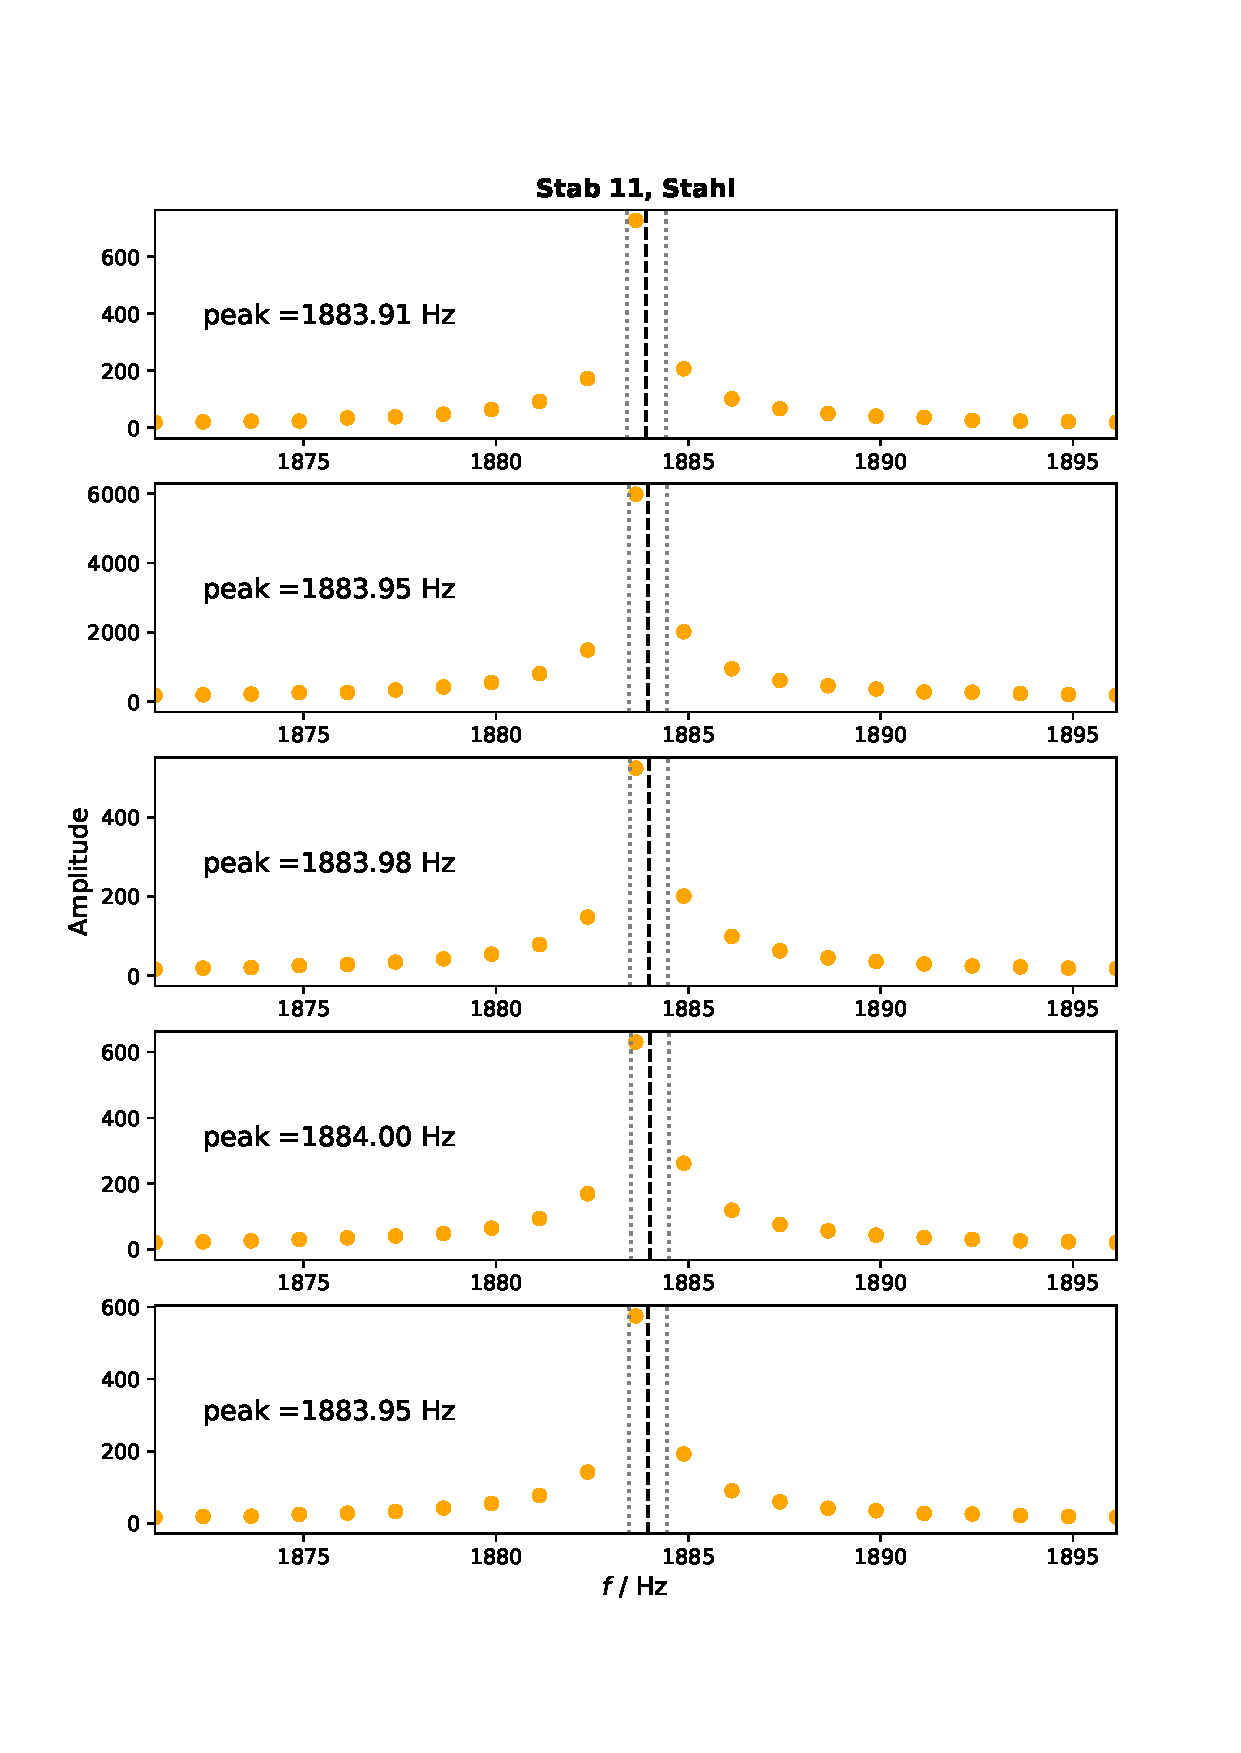
\includegraphics[width=\linewidth]{plots/anhang4.pdf}
\end{figure}

\end{document}
